% Compilation using 'acmsmall.cls' - version 1.3 (March 2012), Aptara Inc.
% Steps to compile: latex, bibtex, latex latex

\documentclass[prodmode,acmtrets]{acmsmall} % Aptara syntax

% Package to generate and customize Algorithm as per ACM style
\usepackage[ruled]{algorithm2e}
%\usepackage{amsmath,epsfig}
%\usepackage[table]{xcolor}
%\usepackage{amsmath,amsfonts,epsfig}
%\usepackage{fancyhdr}
%\usepackage{mathdots,colortbl,dcolumn,rotating,subfigure,appendix}
%\usepackage[scriptsize,it]{caption}
\usepackage{graphicx}
\usepackage{epstopdf}
\usepackage{multirow}
\usepackage{amssymb}
\usepackage[cmex10]{amsmath}
\usepackage[tight,footnotesize]{subfigure}
\usepackage{stfloats}
\usepackage{threeparttable}

%\renewcommand{\algorithmcfname}{ALGORITHM}
\SetAlFnt{\small}
\SetAlCapFnt{\small}
\SetAlCapNameFnt{\small}
\SetAlCapHSkip{0pt}
\IncMargin{-\parindent}

% Metadata Information for publication
\acmVolume{0}
\acmNumber{0}
\acmArticle{0}
\acmYear{2014}
\acmMonth{0}

% Document starts
\begin{document}

% Page heads
\markboth{K. Shi et al.}{Imprecise Datapath Design: An Overclocking Approach}

% Title portion
\title{Imprecise Datapath Design: An Overclocking Approach}
\author{KAN SHI, DAVID BOLAND\\
and GEORGE A. CONSTANTINIDES
\affil{Imperial College London}
}
\vspace{-5ex}


\begin{abstract}
%Releasing the tight accuracy requirement would potentially offer greater freedom to create a design with better performance or energy efficiency.
In this paper, we describe an alternative circuit design methodology when considering trade-offs between accuracy, performance and silicon area. We compare two different approaches that could trade accuracy for performance. One is the traditional approach where the precision used in the datapath is limited to meet a target latency. The other is a proposed new approach which simply allows the datapath to operate without timing closure. We demonstrate analytically and experimentally that on average our approach obtains either smaller errors or equivalent faster operating frequencies in comparison to the traditional approach. This is because the worst case caused by timing violations only happens rarely, while precision loss results in errors to most data. We also show that for basic arithmetic operations such as addition, applying our approach to the simple building block of ripple carry adders can achieve better accuracy or performance than using faster adder designs to achieve similar latency.
\end{abstract}

\category{B.8.2}{Performance and Reliability}{Performance Analysis and Design Aids}

\terms{Design Methodologies, Overclocking, FPGA, Performance Modeling and Analysis}

\keywords{Approximate Computing, Truncation, Imprecise Design}

\acmformat{Kan Shi, David Boland,
and George A. Constantinides, 2013. Imprecise Datapath Design: An Overclocking Approach.}

\begin{bottomstuff}
This work is supported by the EPSRC, under
grant EP/I020557/1 and grant EP/I012036/1.

Author's addresses: K. Shi, D. Boland {and} G. A. Contantinides,
Department of Electrical and Electronic Engineering,
Imperial College London.
\end{bottomstuff}

\maketitle


\section{Introduction}
%With the continuous scaling of CMOS technology to the nanometer regime, circuit performance has increased tremendously over the past decades. However, the drastic variations introduced by higher integration densities is anticipated to be the major obstacle when designing reliable, high performance circuits. Currently, hardware designers tend to employ conservative safety margins to ensure a uniform functionality across a variety of possible working environments. Nevertheless, continuing with this approach could become very costly in the short term future. This is because the highly scaled CMOS devices would inevitably exhibit probabilistic or statistical behavior, meaning that we can no longer expect a uniform circuit performance. Furthermore, covering all possible worst cases would become increasingly difficult, expensive and result in large yield loss because of the variation.

Performance is a critical issue when designing embedded computing systems. Specifically, a large volume of current studies has demonstrated that significant performance gains can be achieved by FPGA-based accelerators over software designs across a wide range of applications~\cite{UnderwoodFPGAvsCPU,David_MINRES}. However, one of the major factors that limits the performance of these accelerators is that they typically run at much lower clock frequencies than general purpose processors (GPPs) or graphics processing units (GPUs).

In order to boost the operating frequency of a datapath, the standard approaches are either to heavily pipeline the design or to reduce the precision throughout the datapath. For the former method, it should be noted that assuming perfect pipeline stage balancing, further pipelining will not tend to reduce the latency of the datapath. As a result, this method will not be applicable to many embedded applications, which often have strict latency requirements, or in any datapath containing feedback where C-slow retiming is inappropriate. For the second approach, reducing the datapath precision would reduce the latency at the cost of introducing quantization errors into the design. This has inspired research into exploiting the potential benefits of using the minimum precision necessary to satisfy a certain accuracy or performance specification~\cite{GeorgeDT11}. A brief review of existing approaches in this area will be discussed in Section~\ref{Section_Background_WL}.

Unfortunately, neither of these conventional approaches tends to remove the conservative safety margin, which is introduced to ensure a uniform functionality across a variety of possible working environments. Nevertheless, continuing with employing the guard-bands to cover all worst cases would become increasingly difficult and expensive in the short-term future, because of the continuous scaling of the process technology. In recent years, we have seen a growth of research that explores the potential power or performance benefits that can be obtained when relaxing the guard-bands~\cite{NewBox2004}. The detailed review of this research field will be presented in Section~\ref{Section_Background_Imprecise}.

In this paper, we describe an alternative circuit design methodology when considering trade-offs between accuracy, performance and silicon area. Since it is unlikely to create a completely error-free design as any data representation would introduce quantization errors, we take a radical shift forward by suggesting that for certain applications it is beneficial to move away from the traditional model of creating a conservative design that is guaranteed to avoid timing violations. Instead, it may be preferable to create a design in which timing violations may occur, under the knowledge that they only occur rarely because specific input patterns are required to generate the worst case errors. This paper elaborates on the prior work~\cite{SKfccm13}, by incorporating silicon area as another evaluation metric. This enables us to find the optimum design choice of the basic arithmetic operators under various design constraints. A summary of the main contributions of this work are as follows:

\vspace{-.5ex}
\begin{itemize}
\item Detailed modeling methods of probabilistic errors generated in basic arithmetic primitives from two design scenarios to trade accuracy for performance: overclocking the datapath or truncating precisions used throughout the datapath,
\item Exploring the accuracy-performance-area trade-offs for key arithmetic operators to illustrate the optimum architecture for a certain arithmetic function under a given requirement of silicon area,
\item Demonstration of the proposed findings analytically and experimentally from FPGA implementations that allowing rare timing violations to happen leads to a reduction of average errors or an improvement of performance over truncating the datapath precisions to meet timing.
\end{itemize}
%\vspace{-2ex}

The rest of this paper is organized as follows: It first reviews in detail the current literature regarding the approaches used in word-length optimization and approximate datapath design in Section~\ref{Section_Background}. The analytical error models for two different adder structures: the ripple carry adder (RCA) and the carry-select adder (CSA), are discussed in Section~\ref{section_RCA} and Section~\ref{Section_CSA}, respectively. The decision of the optimum adder structure under the accuracy-performance-area trade-offs, is then put forward in Section~\ref{Section_OptimumAdder}. It is followed by a description of the probabilistic error models for another arithmetic operator, the constant coefficient multiplier (CCM), in Section~\ref{section_CCM}. Section~\ref{Section_ExpSetup} discusses a practical experimental setup to verify our models and test the proposed design methodology. We then demonstrate the benefits of our proposed approach in Section~\ref{Section_Experiments}. Finally, conclusion of this work and possible future work are discussed in Section~\ref{Section_Conclusion}.
%discusses the conclusions of this work and the possible research directions in the future.

\section{Background}\label{Section_Background}
\subsection{Word-length Optimization}\label{Section_Background_WL}
There exists a significant amount of work demonstrating that optimizing the datapath precision would bring a substantial benefits on clock speed, silicon area and power consumption. There are two main research directions in this area. The first discusses methods to analyze the errors caused by the usage of finite precision and compute bounds on the worst-case errors seen at the output of the design. Related techniques include the simulation-based approach~\cite{SungWLop_Simulation} and the analytical-based approach such as interval arithmetic~\cite{moore1966IA}, affine arithmetic~\cite{de2004affine}, Satisfiability-Modulo Theories~\cite{SAT2010} and polynomial representations~\cite{Boland2011TCAD}. A detailed summary of these methods can be found in~\cite{GeorgeDT11}. In the second research field, these tools are utilized to choose the minimum precision within a datapath to satisfy a required accuracy specification~\cite{RoldaoWLop_Simulation}. In this work, two different design scenarios are analyzed. In the conventional scenario, we speculate and reduce the original word-length in the datapath under a given timing constraint while ensuring no timing errors will occur. In the proposed new scenario, we operate the datapath with the original word-length while allowing timing violations sometimes to happen. The truncation errors derived in the former scenario are then compared to the overclocking errors generated in our proposed new scenario.

%we speculate and employ the maximum word-length in the datapath under a given timing constraint while ensuring no timing errors will occur. The truncation errors derived in this process are then compared to the overclocking errors generated in our proposed new scenario.

\subsection{Imprecise Circuit Design Methodology}\label{Section_Background_Imprecise}
It is worth noting that the choice of precision is not the only source of error when designing a datapath. Recently we have seen a growth of parallel streams of research which aim at exploring alternative methods to trade accuracy for design efficiency. This strand of research is motivated by the fact that extra benefits of manufacturing, test, power and timing can be obtained if the tight requirement of absolute correctness is released for devices and interconnects, as pointed out by the International Technology Roadmap for Semiconductors (ITRS) in 2007~\cite{semiconductor2007international}. This topic is expected to be of growing importance in the future, because we will face new design challenges as the technology scales further.

According to the existing literature, one way to operate circuits beyond the deterministic region is to relax the design constraints and the guard-bands that are conventionally used to avoid the worst cases. A series of work known as ``Better-Than-Worst-Case (BTWC) Design'' introduced a universal framework to push the circuit performance to its limits~\cite{BetterThanWS2005}. In general, a BTWC design is composed of cores and checkers. The cores are operated with high performance by eliminating the guard-bands, meanwhile the possible timing errors are diagnosed by the checkers. Optionally the system can be recovered at the observation of errors. As an exemplary design, the Razor project~\cite{Razor2003,Razor2004} was proposed to shave the conservative timing margins by overcalling the supply voltage and clock frequency, while monitoring the output error rates by utilizing a self-checking circuit. This work demonstrated that the benefits brought by removing the safe margin outweigh the cost of monitoring and recovering from errors. For example, over $30\%$ power consumption can be saved with $\sim1\%$ error rates at the output, respectively. Related work also includes a similar frequency overcalling technique by operating circuits slightly slower than the critical path delay with dedicated checker circuits to ensure that timing errors will not occur~\cite{TEAtime2004}, or developing timing analysis tools that decide the optimum operating frequencies in the non-deterministic region due to process variation~\cite{ProbabilisticSTA}. However, the major problem of the BTWC work is the extra cost introduced by implementing the checker circuits.
%of silicon area due to the implementation of the checker circuits.

Another field of study has shown that errors can be potentially tolerated in various applications, e.g. DSP applications involving human perception. In this case, even greater performance or power benefits can be achieved, as the design overhead of the checkers can be eliminated. Current research in this area focuses on designing probabilistic or imprecise circuits both at a software level and a hardware level. For instance at the programming language level, a tool was proposed~\cite{EnerJ2011Uwash,Truffle2012Uwash} to divide the program into the precise parts and the approximate parts, which are mapped to different hardware with different speed-grades, supply voltages etc., respectively. This technique enables a relatively high service quality, in the meantime energy reduction can be obtained due to approximation. Similar ideas have also been applied on hardware directly. As an example, Palem et~al.~\cite{NonUniformScaling} described a non-uniform voltage scaling technique for the ripple carry adder. In this study, multiple voltage regions are employed for different bits along a carry chain. That is, higher voltage would be applied for computations generating most significant bits, and vice versa. Nevertheless, utilizing several voltage regions within a ripple carry adder will rarely be practical in real situations. Furthermore, the overhead of applying this technique is not addressed.

While the aforementioned literature take advantage of the fact that only specific input patterns could cause timing errors, research on imprecise architectures take this one step further by designing simplified circuits for performance and/or energy efficiency. For example, Lu et~al. proposed a ``shrinking'' datapath that can be utilized to mimic and speculate the original logic functions~\cite{IntelSpeeding}. Kulkarni et~al. described an under-designed $2\times2$ multiplier unit, of which the worst case was replaced by a normal case based on the straightforward Karnaugh-Map analysis~\cite{Undersigned2x2multiplier}. In both cases, reduction of area and power consumption can be achieved at the cost of accuracy. In addition, Gupta et~al. developed approximate adders at the transistor level and compared the energy efficiency of their proposed architectures over truncation of input word-length of conventional structures~\cite{Gupta2013TransCADICS}. However, we should note that using imprecise architectures means correct results would never be obtained for certain input patterns. Another limitation is that the link between the probability of output correctness and energy savings or performance improvements are rarely analyzed in current research. In addition, these techniques cannot be directly applied onto existing hardware platforms such as FPGAs.

In this work, we propose an alternative methodology to remove the limitations of those existing approaches. It is argued in this paper that our method can be easily applied to existing hardware arithmetic operators, and we support this hypothesis analytically by presenting theoretical probabilistic error models, and experimentally by using FPGAs.

\section{Ripple Carry Adder}\label{section_RCA}
\subsection{Adder Structures in FPGAs}
Adders serve as a key building block for arithmetic operations. In general, the ripple carry adder (RCA) is the most straightforward and widely used adder structure. As such, the philosophy of our approach is first exemplified with the analysis of an RCA. We later describe how this methodology can be extended to other arithmetic operators such as CSAs and CCMs, which are commonly used in DSP applications and numerical algorithms, in Section~\ref{Section_CSA} and Section~\ref{section_CCM} respectively.

Typically the maximum frequency of a RCA is determined by the longest carry propagation delay. Consequently, modern FPGAs offer built-in architectures for very fast ripple carry addition. For instance, the Altera Cyclone series uses fast tables~\cite{AlteraCyclone} while the Xilinx Virtex series employs dedicated multiplexers and encoders for the fast carry logic~\cite{Virtex6}. Fig.~\ref{FPGA adder} illustrates the structure of an $n$-bit RCA, which is composed of $n$ serial-connected full adders (FAs) and utilizes the internal fast carry logic of the Virtex-6 FPGA.

While the fast carry logic reduces the time of each individual carry-propagation delay, the overall delay of carry-propagation will eventually overwhelm the delay of sum generation of each LUT with increasing operand word-lengths. We perform our initial analysis based on the assumption that the carry propagation delay of each FA is a constant value $\mu_c$, which is a combination of logic delay and routing delay. Hence the critical path delay of the RCA is given by~(\ref{Eq:RCA_delay}), as shown in Fig.~\ref{FPGA adder}.
%
\begin{eqnarray}\label{Eq:RCA_delay}
	\mu_{RCA}=n\cdot\mu_c
\end{eqnarray}

For an $n$-bit RCA, it follows that if the sampling period $T_S$ is greater than $\mu_{RCA}$, correct results will be sampled. If, however, faster-than-rated sampling frequencies are applied such that $T_S<\mu_{RCA}$, intermediate results will be sampled, potentially generating errors.

\begin{figure}[t]
  \centering
  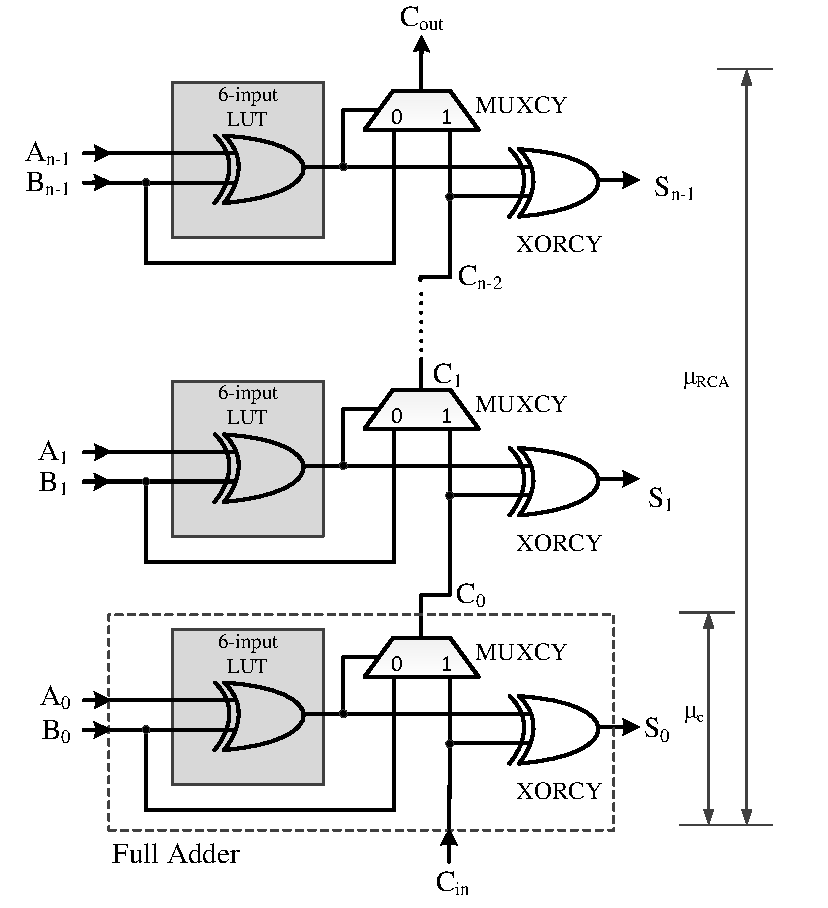
\includegraphics[width=3.2in]{./Figures/FastCarryLogic.pdf}
  %  \vspace{-2ex}
  \caption{An $n$-bit ripple carry adder in the Xilinx Virtex-6 FPGA.}
  \label{FPGA adder}
  %\vspace{-3.5ex}
\end{figure}

In the following sections, we consider two methods that would allow the circuit to run at a frequency higher than $1/{T_S}$. The first is a traditional circuit design approach where operations occur without timing violations. To this end, the operand word-length is truncated in order to meet the timing requirement. This process would result in truncation or roundoff error. In our proposed new design scenario, circuits are implemented with greater word-length, but are clocked beyond the safe region so that timing violations sometimes occur. This process would generate ``overclocking error''.

\subsection{Probabilistic Model of Truncation Error}\label{section_RCA_TruncationError}
For ease of discussion, we assume that the input to our circuit is a fixed point number scaled to lie in the range $[-1,1)$. In our initial analysis, we assume every bit of each input is uniformly and independently generated. However, this assumption will be relaxed in Section~\ref{Section_Experiments} where the predictions are verified using real image data. The errors at the output are evaluated in terms of the absolute value and the probability of their occurrence. These two metrics are combined as the error expectation.

If the input signal of a circuit contains $k$ bits, truncation error occurs when the input signal is truncated from $k$ bits to $n$ bits. Under this premise, the mean value of the truncated bits at signal input ($E_{Tin}$) is given by (\ref{ET at single input}).
%
\begin{eqnarray}\label{ET at single input}
%\small
%\scriptsize
%  \begin{split}
    E_{Tin} = \frac{1}{2}\sum_{i=n+1}^{k}2^{-i} = 2^{-n-1}-2^{-k-1}
%  \vspace{-1ex}
%  \end{split}
\end{eqnarray}

Since we assume there are two mutually independent inputs to the RCA, the overall expectation of truncation error for the RCA is given by (\ref{Eq:TruncationError}).
%
\begin{eqnarray}\label{Eq:TruncationError}
%\small
%\footnotesize
  E_T=\left\{
    \begin{matrix}
        2^{-n}-2^{-k}, & \textrm{if $n<k$}\\
        0, & \textrm{otherwise}
    \end{matrix}
  \right.
\end{eqnarray}
%\normalsize

\subsection{Probabilistic Model of Overclocking Error}
\subsubsection{Generation of Overclocking Error}\label{subsub:Generation of Overclocking Error}
For a given $T_S$, the maximum length of error-free carry propagation is described by~(\ref{Eq:Max_CClength}), where $f_S$ denotes the sampling frequency.
%
\begin{eqnarray}\label{Eq:Max_CClength}
    b := \left\lceil \frac{T_S}{\mu_c} \right\rceil= \left\lceil \frac{1}{\mu_c\cdot f_S}\right\rceil
\end{eqnarray}

However, since the length of an actual carry chain during execution is dependent upon input patterns, in general, the worst case may occur rarely. To determine when this timing constraint is not met and the size of the error in this case, we expand standard results~\cite{DigitalICDesign} to the following statements, which examine carry generation, propagation and annihilation, as well as the corresponding summation results of a single bit $i$ within an $n$-bit RCA ($0\leq i<n$), according to the relationship between its input patterns $A_i$ and $B_i$:
%
 \begin{itemize}
   \item Carry generation: $A_i=B_i=1$, a new carry chain is generated at bit $i$, and $S_i=C_{i-1}$;
   \item Carry propagation: $A_i\neq B_i$, the carry propagates for this carry chain at bit $i$, and $\bar{C_{i-1}}=1$, $S_i=0$;
   \item Carry annihilation: $A_i=B_i$ (either $0$ or $1$), the current carry chain annihilates at bit $i$, and $S_i=C_{i-1}=1$.
 \end{itemize}

 \subsubsection{Absolute Value of Overclocking Error}
For an $n$-bit RCA, let $C_{tm}$ denote the carry chain generated at bit $S_t$ with the length of $m$ bits. For a certain $f_S$, the maximum length of error-free carry propagation, $b$, is determined through (\ref{Eq:Max_CClength}). The presence of overclocking error requires $m>b$. Since the length of the carry chain cannot be greater than $n$, parameters $t$ and $m$ are bounded by (\ref{Eq:t_RCA}) and (\ref{Eq:m_RCA}):
%
\begin{align}
%\small
%\footnotesize
%\scriptsize
  \label{Eq:t_RCA}  0&\leq t \leq n-b\\
    b&<m\leq n+1-t      \label{Eq:m_RCA}
%    \vspace{-1ex}
\end{align}

For $C_{tm}$, correct results will be generated from bit $S_t$ to bit $S_{t+b-1}$. Hence the absolute value of error seen at the output, normalized to the MSB, is given by (\ref{Eq:Output_Error}), where $\hat{S_i}$ and $S_i$ denote the actual value and error-free value of outputs at bit $i$, respectively.
%
\begin{eqnarray}\label{Eq:Output_Error}
%\small
%\footnotesize
    e_{tm}=\frac{\left|\sum_{i=t+b}^{n}(S_i-\hat{S_i})\cdot 2^i\right|}{2^n}
%    \vspace{-1ex}
\end{eqnarray}

$S_i$ and $\hat{S_i}$ can be determined using the equations from the previous statements in Section~\ref{subsub:Generation of Overclocking Error}. In the error-free case, the carry will propagate from bit $S_t$ to bit $S_{t+m-1}$, and we will obtain $S_{t+b}=S_{t+b+1}=\cdots=S_{t+m-2}=0$ for carry propagation, and $S_{t+m-1}=1$ for carry annihilation. However, when a timing violation occurs, the carry will not propagate through all these bits. Hence we have $\hat{S}_{t+b}=\hat{S}_{t+b-1}=\cdots=\hat{S}_{t+m-2}=1$ for carry propagation, and $\hat{S}_{t+m-1}=0$ for carry annihilation. Substituting these values into (\ref{Eq:Output_Error}) yields (\ref{Eq:etm}). Interestingly as seen in~(\ref{Eq:etm}), the magnitude of overclocking error has no dependence on the length of carry chain $m$.
%
\begin{eqnarray}\label{Eq:etm}
%\small
%\footnotesize
%  \begin{split}
    e_{tm} = \frac{\left|2^{t+m-1}-2^{t+m-2}-\dots-2^{t+b}\right|}{2^n} = 2^{t+b-n}
%  \end{split}
\end{eqnarray}

\subsubsection{Probability of Overclocking Error}
The carry chain $C_{tm}$ occurs when there is a carry generated at bit $t$, a carry annihilated at bit $t+m-1$ and the carry propagates in between. Consequently, its probability $P_{tm}$ is given by (\ref{Eq:Ptm_RCA_General}).
%
\begin{eqnarray}\label{Eq:Ptm_RCA_General}
    P_{tm}=P_{(A_t=B_t=1,~A_i\neq B_i,~A_{t+m-1}=B_{t+m-1})},~i\in [t+1,t+m-2]
\end{eqnarray}

Under the assumption that $A$ and $B$ are mutually independent and uniformly distributed, (\ref{Eq:Ptm_RCA_General}) can be modified as given in~(\ref{Eq:Ptm_RCA}). Also we have $P_{(A_i=B_i=1)}=1/4$, $P_{(A_i\neq B_i)}=1/2$ and $P_{(A_i=B_i)}=1/2$. Thus $P_{tm}$ can be obtained by~(\ref{Eq:Ptm2}). Note that~(\ref{Eq:Ptm2}) takes into account the carry annihilation always occurs when $t+m-1=n$.
%
\begin{eqnarray}\label{Eq:Ptm_RCA}
%\small
%\footnotesize
  P_{tm}=P_{(A_t=B_t=1)}P_{(A_{t+m-1}=B_{t+m-1})}\cdot \prod_{i=t+1}^{t+m-2}P_{(A_i\neq B_i)}
%  \vspace{-1ex}
\end{eqnarray}
%
\begin{eqnarray}\label{Eq:Ptm2}
%\small
%\footnotesize
    P_{tm}=\left\{\begin{array}{ll}
      (1/2)^{m+1} & \textrm{if $t+m-1<n$}\\
      (1/2)^{m} & \textrm{if $t+m-1=n$}
    \end{array} \right.
%    \vspace{-1ex}
\end{eqnarray}

In addition, note that the probabilistic models for the magnitude and probability of overclocking errors can be easily generalized for any input distributions with mutually independent bits, since (\ref{Eq:Output_Error}) and (\ref{Eq:etm}) are not related to the input distribution, while (\ref{Eq:Ptm_RCA}) can be employed as long as the value of $P_{(A_i=B_i=1)}$ and $P_{(A_i\neq B_i)}$ is known. If there is dependency between input bits, (\ref{Eq:Ptm_RCA_General}) should be used and the probability value of $P_{(A_i=B_i=1)}$ and $P_{(A_i\neq B_i)}$ would change. For instance, if $A_i$ and $B_i$ are not independent, we have $P_{(A_i=1)}=E_{(A_i)}=1/2$ and $P_{(B_i=1)}=E_{(B_i)}=1/2$ separately for uniform distribution, where $E_{(A_i)}$ denotes the expectation of $A_i$. The probability of $A_i=B_i=1$ is then given by (\ref{Eq:P_dependency})~\cite{TransitionProb} where $\sigma_{(A_i)}$ denotes the standard variation of $A_i$ and $\rho_i$ denotes the temporal correlation between the two inputs at the $i^{th}$ bit. $\rho_i=0$ corresponds to the case where bits are uncorrelated.
%
\begin{eqnarray}\label{Eq:P_dependency}
    P_{(A_i=B_i=1)}=E_{(A_i)}E_{(B_i)}+\rho_i\sigma_{(A_i)}\sigma_{(B_i)}
\end{eqnarray}

It can be seen that if $\rho_i=0$ then $P_{(A_i=B_i=1)}=1/4$ as used to derive (\ref{Eq:Ptm2}). Otherwise $\rho_i$ should be determined before employing our models.

\subsubsection{Expectation of Overclocking Error}
Expectation of overclocking error can be expressed by (\ref{Eq:Eo_exp}).
%
\begin{eqnarray}\label{Eq:Eo_exp}
%\small
%\footnotesize
%\scriptsize
    %E_O=\sum_{t=0}^{n-b}\sum_{m=b+1}^{n-t+1}P_{tm}\cdot e_{tm}
    E_O=\sum_{t}\sum_{m}P_{tm}\cdot e_{tm}
%    \vspace{-1ex}
\end{eqnarray}

Using $P_{tm}$ and $e_{tm}$ from (\ref{Eq:etm}) and (\ref{Eq:Ptm2}) respectively, $E_O$ can be obtained in (\ref{Eq:Eo}).
%
\begin{eqnarray}\label{Eq:Eo}
%\small
%\footnotesize
      E_O=\left\{
        \begin{matrix}
            2^{-b}-2^{-n-1}, & \textrm{if $b\leq n$}\\
            0, & \textrm{otherwise}
        \end{matrix}
      \right.
%      \vspace{-1ex}
\end{eqnarray}

\subsection{Comparison between Two Scenarios}\label{section_RCA_Comparison}
In the traditional scenario, the word-length of RCA must be truncated, using $n=b-1$ bits, in order to meet a given $f_S$. The error expectation is then given by (\ref{Eq:Eo_trad_RCA}).
%
\begin{eqnarray}\label{Eq:Eo_trad_RCA}
%\small
%\vspace{-1ex}
%\footnotesize
%\scriptsize
  E_{trad}=2^{-b+1}-2^{-k}
  \vspace{-1ex}
\end{eqnarray}

Overclocking errors are allowed to happen in our proposed new scenario. Therefore the word-length of RCA is set to be equal to the input word-length, that is, $n=k$. Hence we obtain (\ref{Eq:Eo_new_RCA}) according to (\ref{Eq:Eo}).
%
\begin{eqnarray}\label{Eq:Eo_new_RCA}
%\vspace{-1ex}
%\small
%\footnotesize
%\scriptsize
  E_{new}=2^{-b}-2^{-k-1}
%  \vspace{-1ex}
\end{eqnarray}

Comparing (\ref{Eq:Eo_new_RCA}) and (\ref{Eq:Eo_trad_RCA}), we have (\ref{Eq:Comparison RCA}). This equation indicates that by allowing timing violations, the overall error expectation of RCA outputs drops by a factor of 2 in comparison to traditional scenario. This provides the first hint that our approach is useful in practice.
%
\begin{eqnarray}\label{Eq:Comparison RCA}
%\vspace{-1ex}
%\small
%\footnotesize
%\scriptsize
  \frac{E_{new}}{E_{trad}}=\frac{2^{-b}-2^{-k-1}}{2^{-b+1}-2^{-k}}=\frac{1}{2}
\end{eqnarray}

\section{Carry Select Adder}\label{Section_CSA}
\subsection{Introduction}
As seen in~(\ref{Eq:Comparison RCA}), a factor of 2 reduction in error expectation can be achieved by using the proposed approach in RCA. However, implementing our approach costs extra silicon area in comparison to the conventional approach, because we keep the original word-length $k$ in the new scenario instead of truncating to only $b-1$ bits in the traditional scenario. Besides our approach, there are existing approaches that could be employed to trade silicon area for low latency. For instance, alternative adder architectures, such as carry select adder (CSA), have been proposed to boost performance. In a CSA, the carry chain is divided into multiple overlapped stages, while each stage contains two RCAs and two multiplexers, as shown in Fig.~\ref{Fig_CSA_Structure} and Fig.~\ref{Fig_CSA_SingleStage}, respectively. For a given input, two additions are performed simultaneously within a single stage where the carry input is zero and one separately. One of these two results is then selected according to the actual carry input. Although this structure brings performance benefits, it costs extra hardware resources compared to a standard RCA because the carry chain is duplicated. Furthermore, in FPGA technology, multiplexers are expensive to implement. Due to this reason, we explore the trade-offs between silicon area, accuracy and performance of RCA and CSA in this section.
\vspace{-7ex}
\begin{figure}[htbp]
        \centering
        \subfigure[A CSA with $s$ stages.]{
            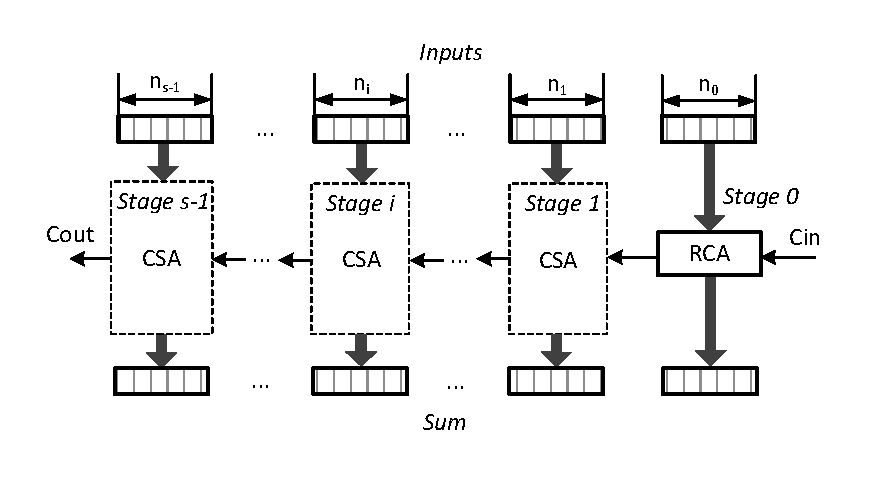
\includegraphics[width=0.6\textwidth]{./Figures/CSA_structure.pdf}
            \label{Fig_CSA_Structure}
        }%\vspace{-2ex}
        \subfigure[The $i^{th}$ stage in the CSA.]{
        \centering
            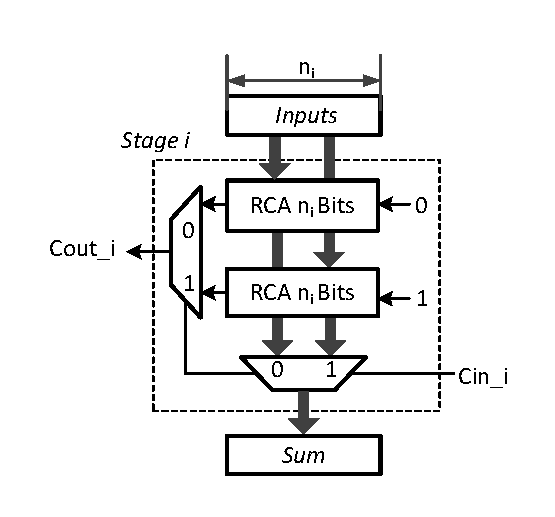
\includegraphics[width=2.2in]{./Figures/CSA_SingleStage.pdf}
            \label{Fig_CSA_SingleStage}
        }
    \vspace{-2ex}
    \caption{The structure diagram of CSA.}
\end{figure}
\vspace{-2ex}

\subsection{Timing Models for Carry Select Adder}
We initially model the CSA in order to understand the relationship between the operating frequency and the maximum word-length of the CSA. This information can then be employed to determine the truncation error based on the models presented in Section~\ref{section_RCA_TruncationError}.

In our analysis, the stage delay of the $i^{th}$ stage in the CSA refers to the combination of the $i$-bit carry propagation delay and the delay of multiplexing the carry from the carry input of the $i^{th}$ stage to the carry output of the CSA. For a CSA with $s$ stages~($s\geqslant 2$), let the stage delay be denoted by $d_{s-1},~\dots,~d_{0}$, where $d_{s-1}$ and $d_{0}$ represent the delay of the most significant and the least significant stages, respectively. We still follow the aforementioned assumption that the critical path delay of the CSA is due to carry propagation and multiplexing the carry output, instead of generating the sum outputs. It should be noted that unlike other stages, the least significant stage of the CSA can be built only by one RCA without multiplexers, since it is directly driven by the carry input. Hence we can obtain the delay of the $i^{th}$ stage as presented in~(\ref{Eq:CSA_SingleStageDelay}), where $\mu_{c}$, $\mu_{mux}$ and $n_i$ denote the delay of $1$-bit carry propagation, the delay of multiplexing and the word-length of the $i^{th}$ stage of the CSA, respectively.
%
\begin{eqnarray}\label{Eq:CSA_SingleStageDelay}
  d_i=\left\{
    \begin{matrix}
      n_i\cdot \mu_{c}+(s-i)\cdot\mu_{mux}, &\textrm{if $i\in\left[1,s-1\right]$}\\
      n_0\cdot \mu_c + (s-1)\cdot\mu_{mux}, & \textrm{if $i=0$}
    \end{matrix}
  \right.
\end{eqnarray}

Under the timing-driven design environment, the delay of each stage of CSA is equalized in order to achieve the fastest operation, as presented in~(\ref{Eq:CSA_DelayEqual}).
%
\begin{eqnarray}\label{Eq:CSA_DelayEqual}
  d_{s-1}=d_{s-2}=\cdots=d_{0}
\end{eqnarray}

In this case, combining~(\ref{Eq:CSA_SingleStageDelay}) and (\ref{Eq:CSA_DelayEqual}) yields $n_i$, which is represented by the word-length of the most significant stage $n_{s-1}$, in (\ref{Eq:CSA_DelayRep}).
%
\begin{eqnarray}\label{Eq:CSA_DelayRep}
 n_i=\left\{
	\begin{matrix}
	  n_{s-1}-(s-1-i)\cdot\frac{\mu_{mux}}{\mu_c}, & \textrm{if $i\in\left[1,s-1\right]$}\\
	  n_{s-1}-(s-2)\cdot\frac{\mu_{mux}}{\mu_c}, &\textrm{if $i=0$}
	\end{matrix}
    \right.
\end{eqnarray}

Sum up $n_i$ to give the total word-length of the CSA in (\ref{Eq:CSA_WL}).
%
\begin{eqnarray}\label{Eq:CSA_WL}
%  \begin{split}
    n_{CSA} =\sum_{i=0}^{s-1}n_{i}= s\cdot n_{s-1}-\frac{\mu_{mux}}{\mu_{c}}\cdot\frac{(s+1)(s-2)}{2}
%  \end{split}
\end{eqnarray}

Conventionally under a given frequency constraint, the word-length of RCA is truncated by using $n_{RCA}=b-1$ bits, where $b$ is determined by~(\ref{Eq:Max_CClength}). Similarly for CSA, the word-length of each stage should be selected in order to satisfy~(\ref{Eq:TimingConstraint_CSA}).
%
\begin{eqnarray}\label{Eq:TimingConstraint_CSA}
  \begin{matrix}
    \forall i\in[0,s-1] &, & d_i\leqslant\frac{1}{f_s}
  \end{matrix}
\end{eqnarray}

Hence for the same frequency requirement, we can form the relationship between the delay of the most significant stage of CSA and the delay of RCA, as given by~(\ref{Eq:WL_MSB_CSA}),
%
\begin{eqnarray}\label{Eq:WL_MSB_CSA}
    \mu_c\cdot (b-1) = n_{s-1}\cdot\mu_c+\mu_{mux}
\end{eqnarray}

Substitute~(\ref{Eq:WL_MSB_CSA}) into (\ref{Eq:CSA_WL}) to replace $n_{s-1}$, we derive the representation of the word-length of CSA in terms of $b$, as presented in~(\ref{Eq:CSA_Timing}).
%
\begin{eqnarray}\label{Eq:CSA_Timing}
  n_{CSA}=s\cdot (b-1)-\frac{\mu_{mux}}{\mu_{c}}\cdot\frac{(s+2)(s-1)}{2}
\end{eqnarray}

\subsection{Accuracy Benefits and Area Overhead in CSA}
We first verify the models for the RCA and CSA in terms of the maximum word-length under the given operating frequencies. For the CSA, the ratio $\mu_{mux}/\mu_c$ can be computed experimentally. We perform post place-and-route simulations on the CSA with 2 stages using Xilinx Virtex-6 FPGA. The delay of the $i^{th}$ stage $d_i$ in~(\ref{Eq:CSA_SingleStageDelay}) is recorded with respect to different word-lengths. The total word-length of CSA can be predicted through~(\ref{Eq:CSA_Timing}). In addition, the maximum word-lengths of the 2-stage CSA and RCA are obtained experimentally by increasing $n_{CSA}$ and $n_{RCA}$ respectively until errors are observed at the output. The comparison between the modeled value and the empirical results is illustrated in Fig.~\ref{Fig_CSA2stage_Timing}. It can be seen that our models for both RCA and CSA match well with the experimental results.
%
%\begin{figure}[htbp]
%        \centering
%        \vspace{-3ex}
%        \subfigure[\scriptsize The modeled value and the experimental results of the maximum word-length of RCA and CSA, with respect to various frequency requirements.]{
%            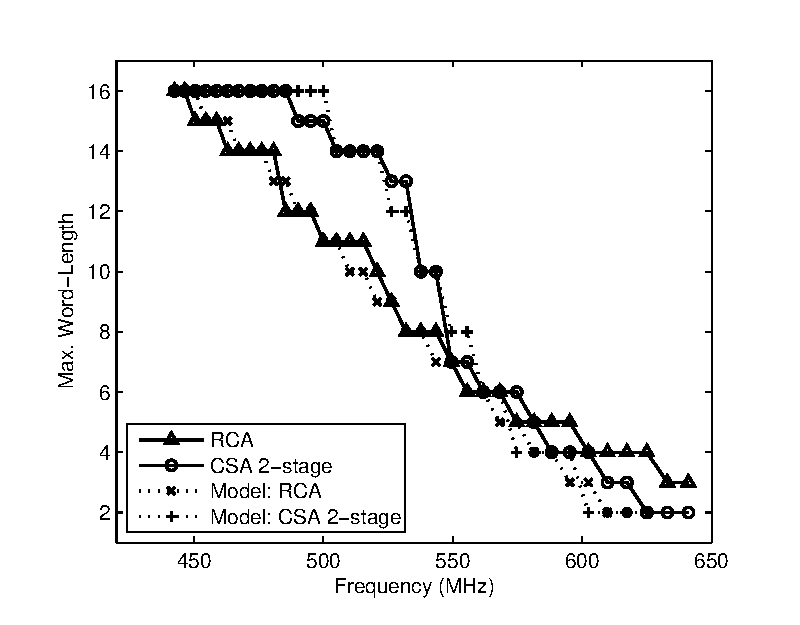
\includegraphics[width=3.5in]{./Figures/CSA2stage_Model_Timing2.eps}
%            \label{Fig_CSA2stage_Timing}
%        }
%        \subfigure[\scriptsize Hardware resource usage for an RCA and a CSA with 2 and 3 stages.]{
%            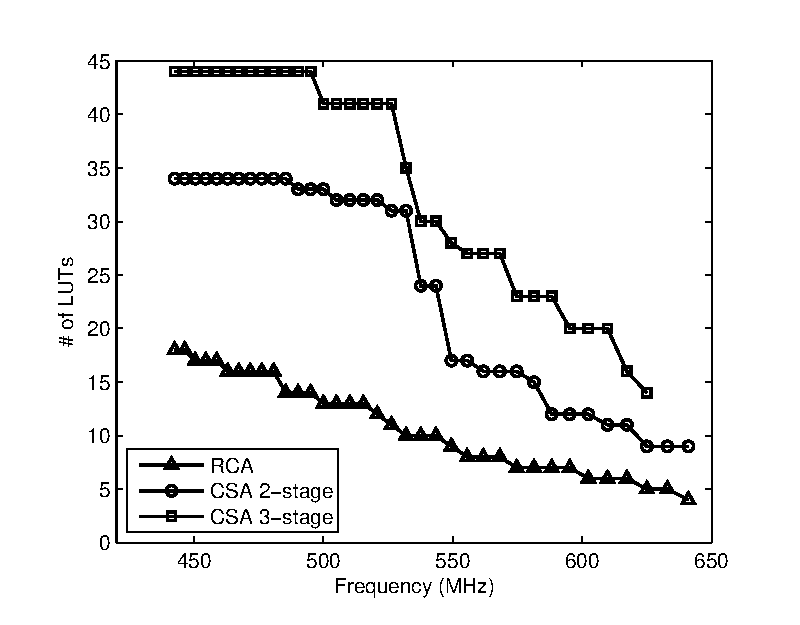
\includegraphics[width=3.5in]{./Figures/CSA3stage_Area2.eps}
%            \label{Fig_CSA3stage_Area}
%        }
%        \vspace{-1.5ex}
%    \caption{A comparison between RCA and CSA in terms of the maximum word-length of input signal and the area consumption.}
%\end{figure}
%
\begin{figure}[t]
    %\centering
    \vspace{-3ex}
    \subfigure[]{
        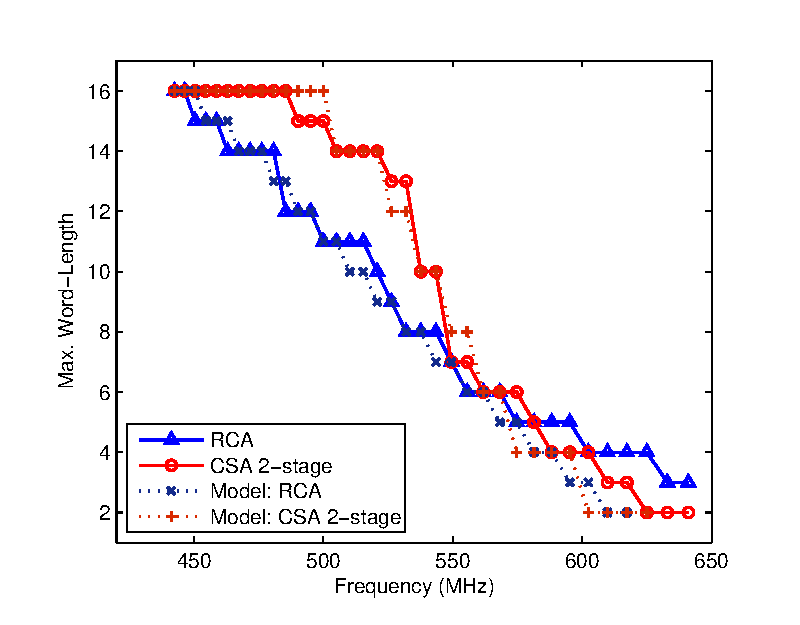
\includegraphics[width=.50\textwidth]{./Figures/CSA2stage_Model_Timing_color.eps}
        \label{Fig_CSA2stage_Timing}
    }%
    \subfigure[]{
        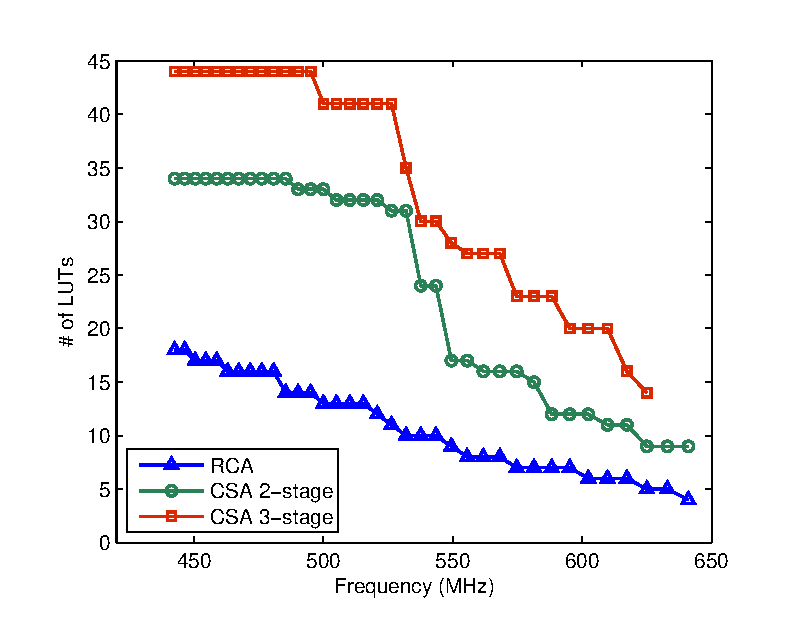
\includegraphics[width=.5\textwidth]{./Figures/CSA3stage_Area_color.eps}
        \label{Fig_CSA3stage_Area}
    }
    \vspace{-2ex}
    \caption{(a) The modeled value and experimental results of the maximum word-length of RCA and CSA, for various frequency requirements. (b) Hardware resource usage for an RCA and a CSA with 2 and 3 stages.}
    \vspace{-1ex}
\end{figure}

Fig.~\ref{Fig_CSA2stage_Timing} also highlights that for a relatively relaxed frequency constraint, the CSA achieves greater word-length than the RCA. This is because the stage parallelism in the CSA enables a greater overall word-length, even though the multiplexer delay limits the word-length of each stage in the CSA when compared to the RCA. When more stringent latency requirement is applied, however, the word-length of each stage is largely limited such that the multiplexer delay becomes comparable to the delay of the carry chain, and this inhibits the benefits of parallelism.

However, the accuracy benefits brought by CSA comes at the cost of a large area overhead. Fig.~\ref{Fig_CSA3stage_Area} depicts the number of LUTs in the FPGA used for an RCA, a 2-stage CSA and a 3-stage CSA. It can be seen that in order to meet a given frequency, the 3-stage CSA consumes $2.4\times\sim3.7\times$ area than RCA, while the 2-stage CSA requires $1.7\times\sim3.1\times$ extra area. This finding poses a question of which is the best adder structure for a specific area budget.

\section{Choosing the Optimum Adder Structure}\label{Section_OptimumAdder}
In Section~\ref{section_RCA}, we discussed two design scenarios for the RCA when considering timing constraints. In this section, we expand our analysis by incorporating silicon area as another evaluation metric, and investigate the accuracy, performance and area trade-offs for different adder structures. In the conventional design scenario, the word-length of RCA and CSA is limited by the given frequency constraint, or/and the available hardware resources. The precision loss potentially generates large errors even without timing violations. However in the new design scenario, we use the RCA with the maximum possible word-length under the given area budget, and the timing constraints are allowed to be violated. This process might result in timing errors as well as truncation errors due to area limitation. We compare these two scenarios with different design goals with the aim of finding the optimum design methodology under each situation.

\subsection{Determination of the Optimum Adder Structure for Given Frequency Requirements}
First, suppose the algorithm designer wished to create a circuit that can run at a given frequency in a given resource constraint while achieving the minimum possible output error. A decision must then be taken over which adder structure achieves this minimum, and whether the structure should be overclocked.

% with the minimum achievable output errors and minimum resource usage, i.e. a pair of $\{Area, Frequency\}$ constraint is applied. In this case, the optimum design method is selected according to the following criteria:

%\begin{itemize}
%  \item Design with the minimum mean value of errors at the output is the optimum design;
%  \item If multiple designs achieve the same accuracy, then the design with minimum area is the optimum design;
%  \item If both the accuracy and area are identical for multiple designs, they are all treated as the optimum design.
%\end{itemize}

As an example slice through the design space, in Fig.~\ref{Fig_CSA_LUT25} we record the mean value of error at outputs with respect to different operating frequencies for both design scenarios when the number of the available LUTs is set to 25. In this graph, we have labeled the optimum adder structure. Note that in this and all the following experiments within this section, in order to apply our models, the input data is randomly generated following the uniform distribution.
%
\begin{figure}[t]
  \centering
  \vspace{-3ex}
  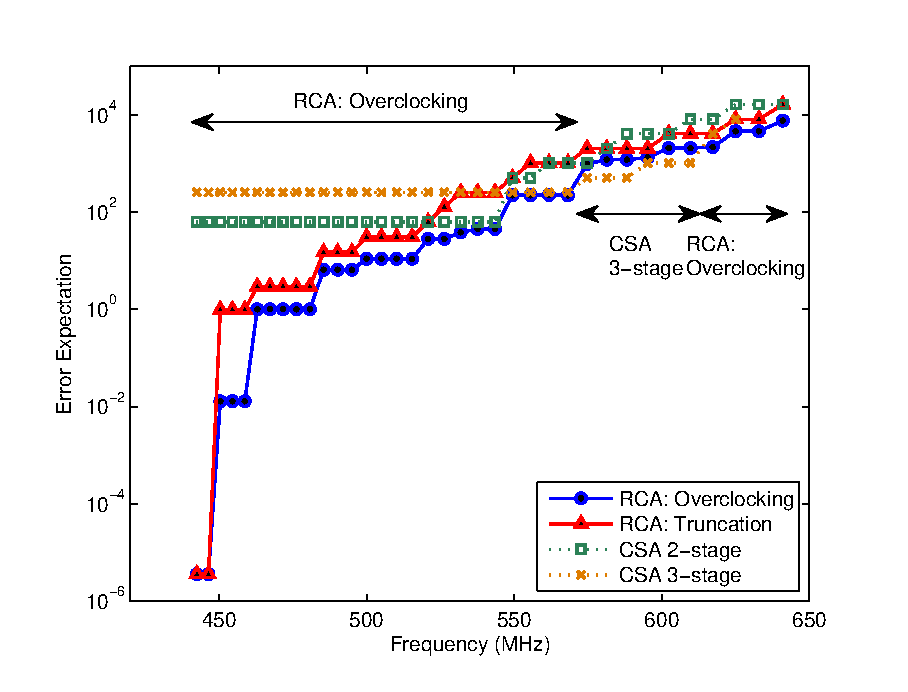
\includegraphics[width=3.3in]{./Figures/Error_LUT25_color.eps}
  \vspace{-2ex}
  \caption{A comparison between two design scenarios when the number of available LUT is 25. The RCA and CSA are investigated in the conventional scenario, while the RCA is explored in the proposed new scenario. The results are obtained from post place-and-route simulations on Xilinx Virtex-6 FPGAs.}
  \vspace{-2ex}
  \label{Fig_CSA_LUT25}
\end{figure}

We first notice from Fig.~\ref{Fig_CSA_LUT25} that for all frequency values, the overclocked RCA achieves no larger error expectation than the RCA with truncated operand word-lengths, as predicted by the models for the RCA in Section~\ref{section_RCA_Comparison}. It can also be observed that the CSA cannot be implemented with the original word-length due to the limited area budget and this leads to large truncation errors. Although the CSA with 3 stages is best for some frequencies, the overclocked RCA is still the optimum design when high operating frequencies are applied.

We then perform similar experiments with a variety of area constraints. We implement CSA with all possible stage numbers within the given area specification. The optimum design methods with respect to different operating frequencies and area consumptions are demonstrated in Fig.~\ref{Fig_CSA_Tradeoff}, from which several observations can be made. Firstly, if the frequency requirement is not large whilst the available area is large enough to implement a CSA in full precision, it will be the optimum design. This is expected from our earlier analysis in Fig.~\ref{Fig_CSA2stage_Timing}. Secondly, the 2-stage CSA is better than the 3-stage CSA and the 4-stage CSA when frequency is low, as it consumes less area although all achieve the same error expectation. Thirdly, it is possible that only part of the CSA can be implemented under a tighter area budget, whereas the RCA still keeps full precision. In this case, area becomes the dominant factor and precision is lost for the CSA, meaning the RCA with overclocking is the optimum design method across almost the whole frequency domain in this situation. Finally, for very stringent area constraints, the word-length of RCA is also limited. This results in truncation errors initially for all design scenarios. However, the RCA with overclocking can still be employed as the optimum design, because it loses less precision than the CSA under the same area constraint.
%
\begin{figure}[t]
  \centering
  \vspace{-2.5ex}
  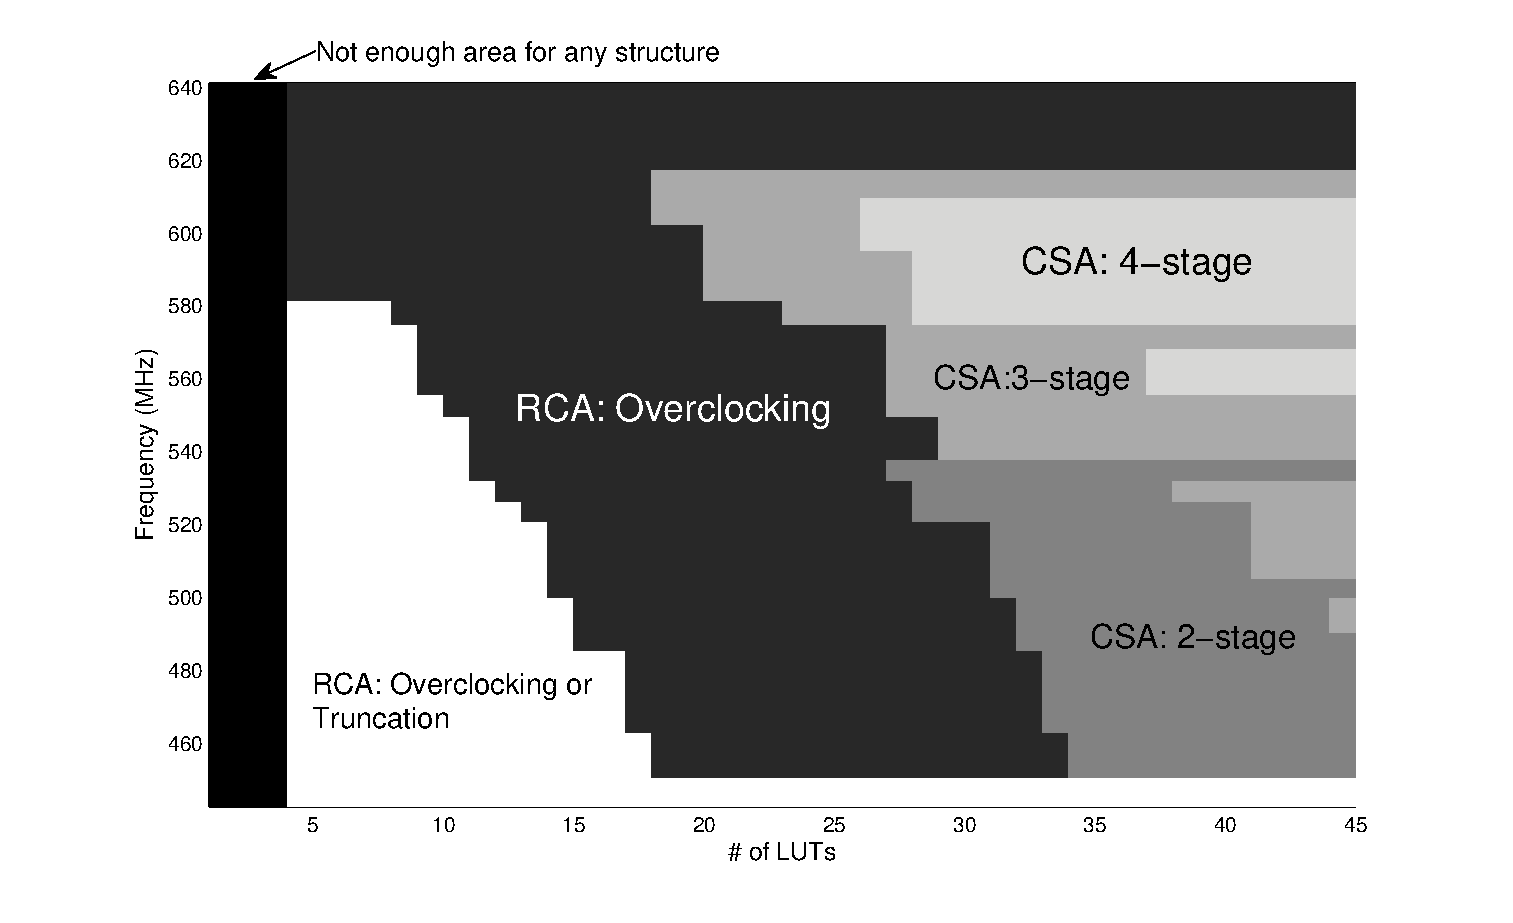
\includegraphics[width=4.5in]{./Figures/Tradeoff_Freq.eps}
  \vspace{-2.5ex}
  \caption{A demonstration of the optimum design methodology which achieves the minimum error at outputs with respect to a variety of frequency and area constraints.}
  \label{Fig_CSA_Tradeoff}
\end{figure}

\vspace{-0.5ex}
\subsection{Determination of the Optimum Adder Structure for Given Accuracy Requirements}
If the design goal is to operate the circuit as fast as possible with the minimum area whilst a certain error budget can be tolerated, the optimum design methodology can be decided as illustrated in Fig.~\ref{Fig_CSA_Tradeoff_Error}. In this situation, the error specifications are evaluated in terms of the mean relative error ($MRE$), as given by~(\ref{Eq:MRE}), where $E_{error}$ and $E_{out}$ refer to the mean value of error and the mean value of outputs, respectively.
%
\begin{eqnarray}\label{Eq:MRE}
  MRE=\left|\frac{E_{error}}{E_{out}}\right|\times 100\%
\end{eqnarray}

In our experiments, $MRE$ is set ranging from $0.001\%$ to $50\%$. For a certain value of $MRE$, the design with the maximum operating frequency is selected as the optimum design. Moreover, the smallest design is the optimum one if multiple structures operate at the same frequency, with a certain area requirement. Fig.~\ref{Fig_CSA_Tradeoff_Error} can thus be obtained based on these criteria.
%
\begin{figure}[t]
    \centering
    \vspace{-2ex}
    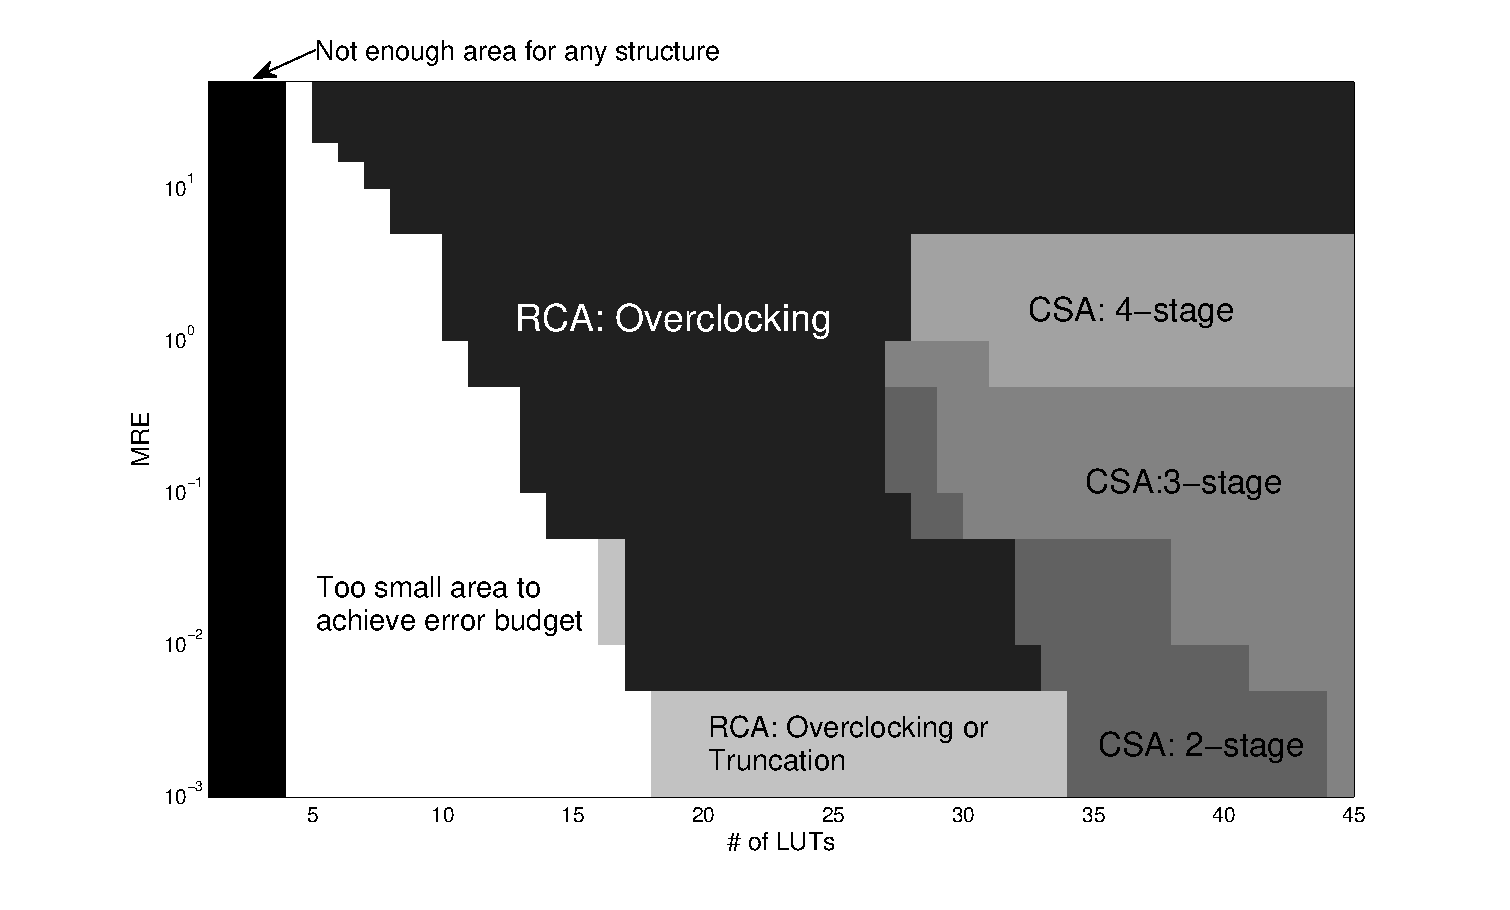
\includegraphics[width=4.5in]{./Figures/Tradeoff_Error2.eps}
    \vspace{-2.5ex}
    \caption{A demonstration of the optimum design methodology which runs at the fastest frequency with respect to a variety of accuracy and area constraints.}
    \label{Fig_CSA_Tradeoff_Error}
    \vspace{-1ex}
\end{figure}

For a tight accuracy requirement, e.g. $MRE<0.005\%$, CSA serves as the optimum design choice for large area constraints, as it intrinsically operates faster than RCA. Once again, when the area budget shrinks, the RCA performs best because the precision of the CSA is limited. Similarly to the results in Fig.~\ref{Fig_CSA_Tradeoff}, we see that the overclocked RCA achieves the fastest operating frequencies under most area constraints when the accuracy requirement is released.

\subsection{Design Guidance}
To sum up, the experiments reveal that for both design goals, the CSA is not competitive with the overclocking approach unless one has very relaxed area budget. As a result, for the remainder of this paper, we will focus on the RCA in our following analysis and experiments.

% is the best option only when there is enough hardware resources. However for the remainder of this paper, we are interested in cases where there is a limited area budget, as may be the case in the embedded applications. Due to this reason, we will focus on the RCA in our following analysis and experiments.

\section{Constant Coefficient Multiplier}\label{section_CCM}

As another key primitive of arithmetic operations, CCM can be implemented using RCA and shifters. For example, operation $B=9A$ is equivalent to $B=A+8A=A+(A<<3)$, which can be built using one RCA and one shifter. We first focus on a single RCA and single shifter structure. We describe how more complex structures consisting of multiple RCAs and multiple shifters can be built in accordance with this baseline structure in Section~\ref{CCM_Multi}.

In this CCM structure, let the two inputs of the RCA be denoted by $A_S$ and $A_O$ respectively, which are both two's complement numbers. $A_S$ denotes the ``shifted signal", with zeros padded after LSB, while $A_O$ denotes the ``original signal" with MSB sign extension. For an $n$-bit input signal, it should be noted that an $n$-bit RCA is sufficient for this operation, because no carry will be generated or propagated when adding with zeros, as shown in Fig.~\ref{CCM_fig}.
%
\begin{figure}[htbp]
  \vspace{-5ex}
  \centering
  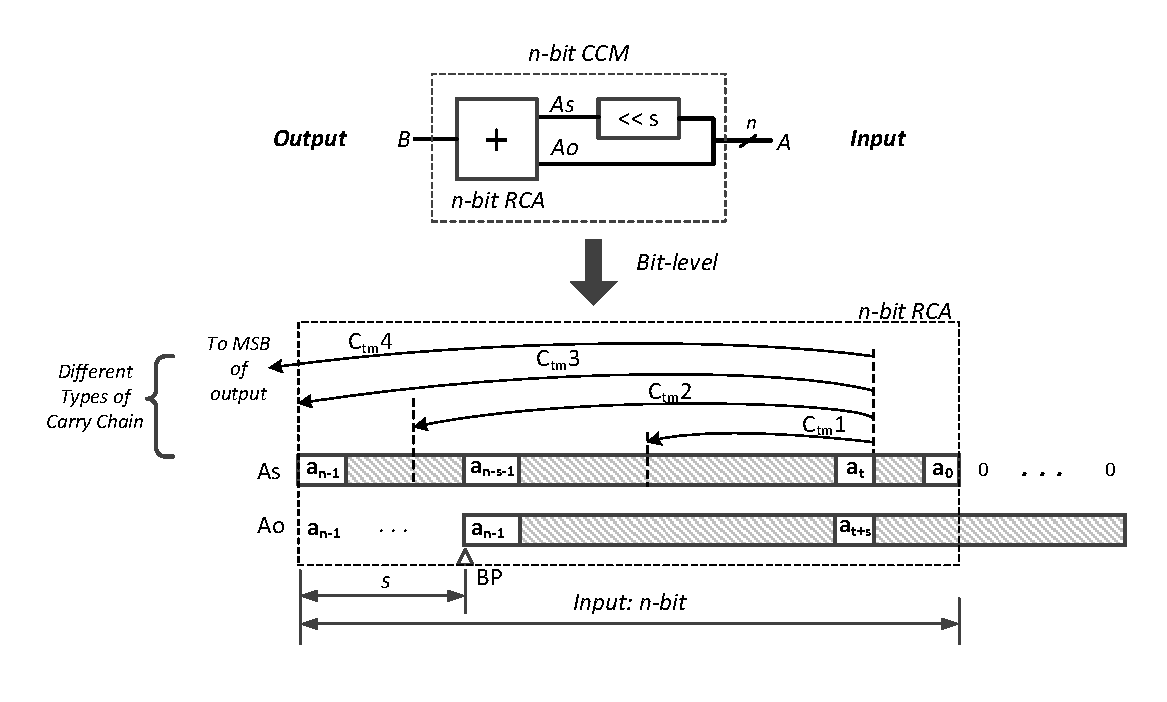
\includegraphics[width=\textwidth]{./Figures/CCM_CarryChain.pdf}
  \vspace{-6ex}
  \caption{Four possible carry chain types in a constant coefficient multiplier with $n$-bit inputs. The notion $s$ denotes the shifted bits and $BP$ denotes the binary point.}
  \label{CCM_fig}
  \vspace{-4ex}
\end{figure}

\subsection{Probabilistic Model of Truncation Error}
Let $E_{Tin}$ and $E_{Tout}$ denote the expectation of truncation error at the input and output of CCM respectively. We then have (\ref{Eq:Et_CCM}), where $coe$ denotes the coefficient value of the CCM, and $E_{Tin}$ can be obtained according to~(\ref{Eq:TruncationError}).
%
\begin{eqnarray}\label{Eq:Et_CCM}
%\vspace{-1ex}
%\small
%\footnotesize
%\scriptsize
  E_{Tout}=|coe|\cdot E_{Tin}
%  \vspace{-1ex}
\end{eqnarray}

\subsection{Probabilistic Model of Overclocking Error}
\subsubsection{Absolute Value of Overclocking Error}
The absolute value of overclocking error of carry chain $C_{tm}$ is increased by a factor of $2^s$ due to shifting, when compared to RCA. Hence $e_{tm}$ in CCM can be modified from (\ref{Eq:etm}) to give (\ref{Eq:etm_CCM}).
%
\begin{eqnarray}\label{Eq:etm_CCM}
%\vspace{-1ex}
%\small
%\footnotesize
  e_{tm}=2^{t+b-n+s}
%  \vspace{-1.5ex}
\end{eqnarray}

\subsubsection{Probability of Overclocking Error}
Due to the dependencies in a CCM, carry generation requires $a_t=a_{t-s}=1$, propagation and annihilation of a carry chain is best considered separately for four types of carry chain generated at bit~$t$. We label these by $C_{tm}1$ to $C_{tm}4$ in Fig.~\ref{CCM_fig}, defined by the end region of the carry chain. For $C_{tm}1$, we have:

\begin{itemize}
  \item Carry propagation: $a_i\neq a_{i+s}$ where $i\in[t+1,n-s-2]$;
  \item Carry annihilation: $a_j=a_{j+s}$ where $j\in[t+1,n-s-1]$.
\end{itemize}

Similarly for $C_{tm}2$, we have:

\begin{itemize}
  \item Carry propagation: $a_i\neq a_{n-1}$ where $i\in[n-s-1,n-3]$; or $a_i\neq a_{i+s}$ where $i\in[t+1,n-s-2]$;
  \item Carry annihilation: $a_j=a_{n-1}$ where $j\in[n-s-1,n-2]$.
\end{itemize}

For the first two types of carry chain $C_{tm}1$ and $C_{tm}2$, the probability of carry propagation and annihilation is $1/2$ and the probability of carry generation is $1/4$, under the premise that all bits of input signal are mutually independent. Therefore (\ref{Eq:Ptm_CCM1}) can be obtained by substituting this into~(\ref{Eq:Ptm_RCA}).
%
\begin{eqnarray}\label{Eq:Ptm_CCM1}
%\vspace{-1ex}
%\small
%\footnotesize
  P_{tm}=\left(1/2\right)^{m+1}, & \textrm{if $t+m-1\leqslant n-2$}
\end{eqnarray}

For carry annihilation of $C_{tm}3$, it requires $a_{n-1}=a_{n-1}$, which is always true. Thus the probability of $C_{tm}3$ is given by (\ref{Eq:Ptm_CCM2}).
%
\begin{eqnarray}\label{Eq:Ptm_CCM2}
%\vspace{-1ex}
%\small
%\footnotesize
  P_{tm}=\left(1/2\right)^m, & \textrm{if $t+m-1=n-1$}
%  \vspace{-1ex}
\end{eqnarray}
%\normalsize
$C_{tm}4$ represents carry chain annihilates over $a_{n-1}$, therefore carry propagation requires $a_{n-1}\neq a_{n-1}$. This means $C_{tm}4$ never occurs in a CCM.

Altogether, $P_{tm}$ for a CCM is given by (\ref{Eq:Ptm_CCM}).
%
\begin{eqnarray}\label{Eq:Ptm_CCM}
%\small
  P_{tm}=\left\{\begin{array}{ll}
      (1/2)^{m+1} & \textrm{if $t+m-1<n-1$}\\
      (1/2)^{m} & \textrm{if $t+m-1=n-1$}
    \end{array} \right.
    %\vspace{-1ex}
\end{eqnarray}

\subsubsection{Expectation of Overclocking Error}
Since the carry chain of a CCM will not propagate over $a_{n-1}$, the upper bound of parameter $t$ and $m$ should be modified from (\ref{Eq:t_RCA}) and (\ref{Eq:m_RCA}) to give (\ref{Eq:t_CCM}) and (\ref{Eq:m_CCM}).
%
\begin{eqnarray}
%\vspace{-1ex}
%\small
%\footnotesize
%\scriptsize
  \label{Eq:t_CCM} 0\leqslant t\leqslant n-b-1\\
  \label{Eq:m_CCM} b<m\leqslant n-t
%  \vspace{-1ex}
\end{eqnarray}

Finally, by substituting (\ref{Eq:Ptm_CCM}) and (\ref{Eq:etm_CCM}) with modified bounds of $t$ and $m$ into (\ref{Eq:Eo_exp}), we obtain the expectation of overclocking error for a CCM to be given by (\ref{Eq:Eo_CCM}).
%
\begin{eqnarray}\label{Eq:Eo_CCM}
%\vspace{-1ex}
%\small
%\footnotesize
      E_O=\left\{
        \begin{matrix}
            2^{s-b-1}-2^{s-n-1}, & \textrm{if $b\leq n-1$}\\
            0, & \textrm{otherwise}
        \end{matrix}
      \right.
%      \vspace{1ex}
\end{eqnarray}

\subsection{CCM with Multiple RCAs and Shifters}\label{CCM_Multi}
In the case where a CCM is composed of two shifters and one RCA, such as operation $B=20A=(A<<2)+(A<<4)$, let the shifted bits be denoted as $s_1$ and $s_2$ respectively. Hence the equivalent $s$ in (\ref{Eq:Eo_CCM}) can be obtained through~(\ref{Eq:ShiftNo}).
%
\begin{eqnarray}\label{Eq:ShiftNo}
%\footnotesize
%\scriptsize
  s=\left|s_1-s_2\right|
%  \vspace{-1ex}
\end{eqnarray}

For those operations such as $B=37A=(A<<5)+(A<<2)+(A<<1)$, the CCM can be built using a tree structure. Each root node is the baseline CCM and the errors are propagated through an adder tree, of which the error can be determined based on our previous RCA model.

\section{Test Platform}\label{Section_ExpSetup}
In our experiments, we compare two design perspectives. In the first scenario, the word-length of the input signal is truncated before propagating through the datapath in order to meet a given latency. In our proposed overclocking scenario, the circuit is overclocked while keeping the original operand word-length. The benefits of the proposed methodology are demonstrated over a set of DSP example designs, which are implemented on the Xilinx ML605 board with a Virtex-6 LX240T-1 FPGA.

\subsection{Experimental Setup} \label{sub:experimental_setup}
We initially build up a test framework on an FPGA. The general architecture is depicted in Fig.~\ref{Test Framework}. The main body of the test framework consists of the circuit under test (CUT), the test frequency generator and the control logic, as shown in the top dotted box in Fig.~\ref{Test Framework}. The I/Os of the CUT are registered by the launch registers (LRs) and the sample registers (SRs), which are all triggered by the test clock. Input test vectors are stored in the on-chip memory during initialization. The results are sampled using Xilinx ChipScope. Finally, we perform an offline comparison of the output of the original circuit at the rated frequency with the output of the overclocked as well as the truncated designs using the same input vectors.
%
\begin{figure}[htbp]
  \centering
  \vspace{-3.5ex}
  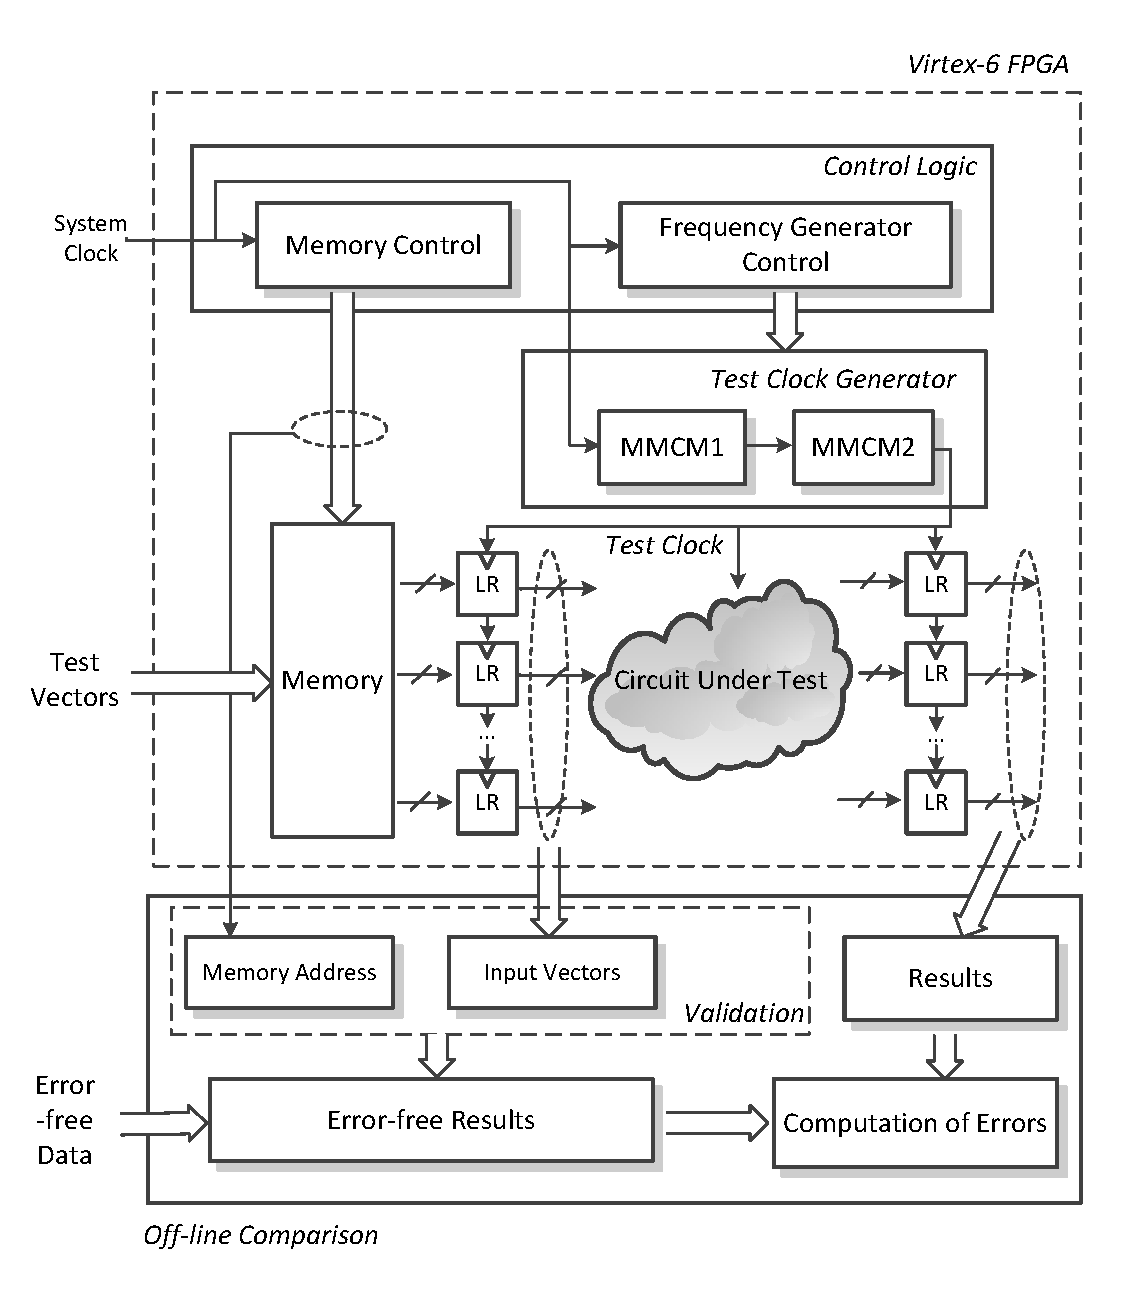
\includegraphics[width=3.7in]{./Figures/TestFramework.pdf}
  \vspace{-1.5ex}
  \caption{Test framework, which is composed of a measurement architecture (the top dotted box) on an FPGA and an off-line comparator using software. The error-free data are obtained by either pre-computation or initial run with low frequencies.}
  \label{Test Framework}
  \vspace{-1.5ex}
\end{figure}

The test frequency generator is implemented using two cascaded mixed-mode clock managers (MMCMs), created using Xilinx Core Generator~\cite{Virtex6Clocking}. Besides the outputs, the corresponding input vectors and memory addresses are also recorded into the comparator, as can be seen in Fig.~\ref{Test Framework}, in order to ensure that the recorded errors arise from overclocking the CUT rather than the surrounding circuitry when high test frequencies are applied.

\subsection{Benchmark Circuits}
Three types of DSP designs are tested: digital filters (FIR, IIR and Butterworth), a Sobel edge detector and a direct implementation of a Discrete Cosine Transformation (DCT). The filter parameters are generated through MATLAB filter design toolbox, and they are normalized to integers for implementation. Table~\ref{Rated_Frequency_table} summarizes the operating frequency of each implemented design in Xilinx ISE14.1 when the word-length of the input signal is 8-bit.
%
\begin{table}[htbp]%
\vspace{-1ex}
\tbl{Rated Frequencies of example Designs.\label{Rated_Frequency_table}}{%
\begin{tabular}{|c|c|c|}
\hline
Design & Frequency (MHz) & Description\\
\hline
FIR Filter & 126.2 & $5^{th}$ order\\
Sobel Edge Detector & 196.7 & $3\times 3$\\
IIR Filter & 140.3 & $7^{th}$ order\\
Butterworth Filter & 117.1 & $9^{th}$ order\\
DCT & 176.7 & 4-point\\
\hline
\end{tabular}}
\end{table}%

The input data are generated from two sources. One is called ``uniform independent inputs'', which are randomly sampled from a uniform distribution of 8-bit numbers. The other is referred to as ``real inputs'', which denote 8-bit pixel values of the $512\! \times\! 512$ Lena image.

\subsection{Correcting for Conservative Timing Margin} % (fold)
\label{sub:exploring_the_conservative_timing_margin}

Generally, the operating frequency provided by EDA tools tends to be conservative to ensure the correct functionality under a wide range of operating environments and workloads. In a practical situation, this may result in a large gap between the predicted frequency and the actual frequency under which the correct operation is maintained~\cite{gojman2013FPGA}.

For example, the frequencies predicted by Xilinx ISE and the actual frequencies of a $5^{th}$~order FIR filter using different word-lengths are depicted in Fig.~\ref{Fig:TimingMargin}. The ``actual'' maximum frequencies are computed by increasing the operating frequency from the rated value until errors are observed at the output; the maximum operating frequency with correct output is recorded for the current word-length. As can be seen in Fig.~\ref{Fig:TimingMargin}, the circuit can operate without errors at a much higher frequency in practice than predicted according to our experiments. A maximum speed differential of $3.2\times$ is obtained when the input signal is 5-bit.
%
\begin{figure}[ht]
  \centering
  \vspace{-2ex}
  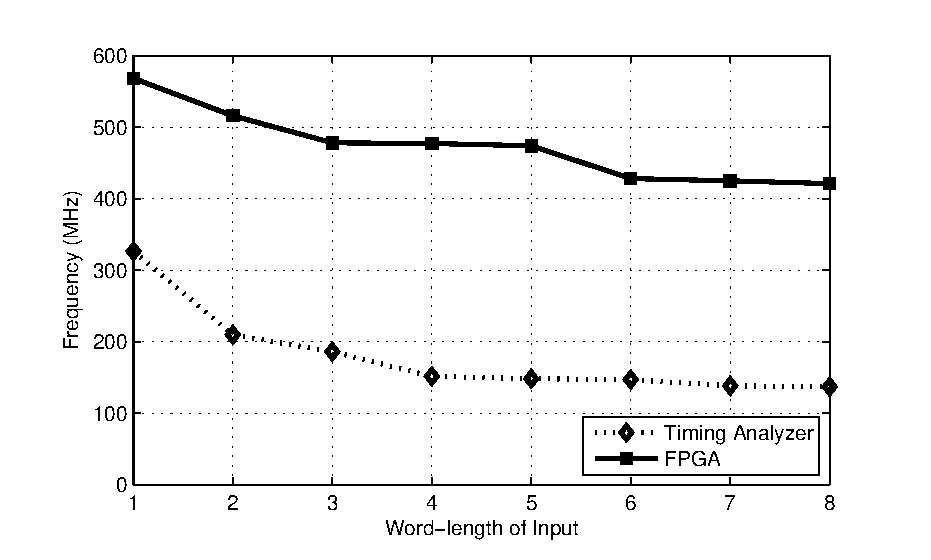
\includegraphics[width=3.2in]{./Figures/Exp/FIR/RatedFrequency3.eps}
  \vspace{-1ex}
  \caption{The maximum operating frequencies for different input word-lengths of an FIR filter. The dotted line depicts the rated frequency reported by the timing analysis tool. The solid line is obtained through real FPGA tests using our platform.}
  \label{Fig:TimingMargin}
  \vspace{-.5ex}
\end{figure}

In our experiments in Section~\ref{Section_Experiments}, the conservative timing margin is removed in the traditional scenario for a fairer comparison to the overclocking scenario. To do this, for each truncated word-length, we select the maximum frequency at which we see no overclocking error on the FPGA board in our lab. For example, in Fig.~\ref{Fig:TimingMargin}, the operating frequency of the design when the word-lengths are truncated to 8,~5 and 2 bits are 400MHz,~450MHz and 500MHz respectively.

Fig.~\ref{Fig:TimingMargin} also demonstrates that when the circuit is truncated, it allows the circuit to operate at a higher frequency than the frequency of full precision implementation. However, a non-uniform period change can be observed for both results. For instance, the maximum operating frequency remains almost constant when the operand word-length reduces from 8 to 6 or from 5 to 3 in both the experimental results and those of timing analyzer. This will cause a slight deviation between our analytical model which assumes that the single bit carry propagation delay to be a constant value, as discussed in (\ref{Eq:Eo_trad_RCA}) with expression $n=b-1$. This deviation will be influenced by many factors such as how the architecture has been packed onto LUTs and CLBs. In addition, process variation might cause non-uniform interconnection delays~\cite{FPGAPV}. However, we shall see that our model remains close to the true empirical results in Section~\ref{Section_Experiments}.

\subsection{Computing Model Parameters}
The accuracy of our proposed models is examined with practical results on Virtex-6 FPGA. We first determine the model parameters. There are two types of parameters in the models of overclocking error. The first is based on the circuit architecture. For example, the word-length of RCAs and CCMs ($n$), the shifted bits of the shifters in CCM ($s$), and the word-length of the input signal ($k$). This is determined through static analysis. The second depends on timing information, such as the single bit carry propagation delay $\mu_c$. In order to keep consistency with the assumption made in models that $\mu_c$ is a fixed value, it is obtained according to the actual FPGA measurement results.

Initially the maximum error-free frequency $f_0$ is applied. In this case we have~(\ref{Eq_decideMu_0}) where $d_c$ is a constant value which denotes the interconnection delay, and $d_0=1/f_0$. The frequency is then increased such that~(\ref{Eq_decideMu_1}) is obtained. This process repeats until the maximum frequency $f_{n-1}$ is applied in~(\ref{Eq_decideMu_2}). Based on these frequency values, $\mu_c$ can be determined.
%
\begin{eqnarray}\label{Eq_decideMu_0}
  %\frac{1}{f_0} &= n\mu+d_c
  d_0 &= n\mu_c+d_c
  \vspace{-13ex}
\end{eqnarray}
\vspace{-4ex}
\begin{align}\label{Eq_decideMu_1}
  d_1 &= (n-1)\mu_c+d_c    \\
  &\cdots               \notag
  \vspace{-3ex}
\end{align}
\vspace{-4ex}
\begin{eqnarray}\label{Eq_decideMu_2}
  {d_{n-1}} &= \mu_c+d_c
\end{eqnarray}

\section{Results and Discussion}\label{Section_Experiments}
\subsection{Case study: FIR filter}
We first assess the accuracy of our proposed models of errors. We record the value of $MRE$ based on (\ref{Eq:MRE}) in a $5^{th}$~order FIR with respect to different operating frequencies. The modeled values of both overclocking error and truncation error of the FIR filter are presented in Fig.~\ref{Fig:FIR} (dotted lines), as well as the actual measurements on the FPGA (solid lines) with two types of input data. The results demonstrate that our models match well with the practical results obtained using the uniform independent inputs.
% FIR
\begin{figure}[tbp]
  \centering
  \vspace{-3ex}
  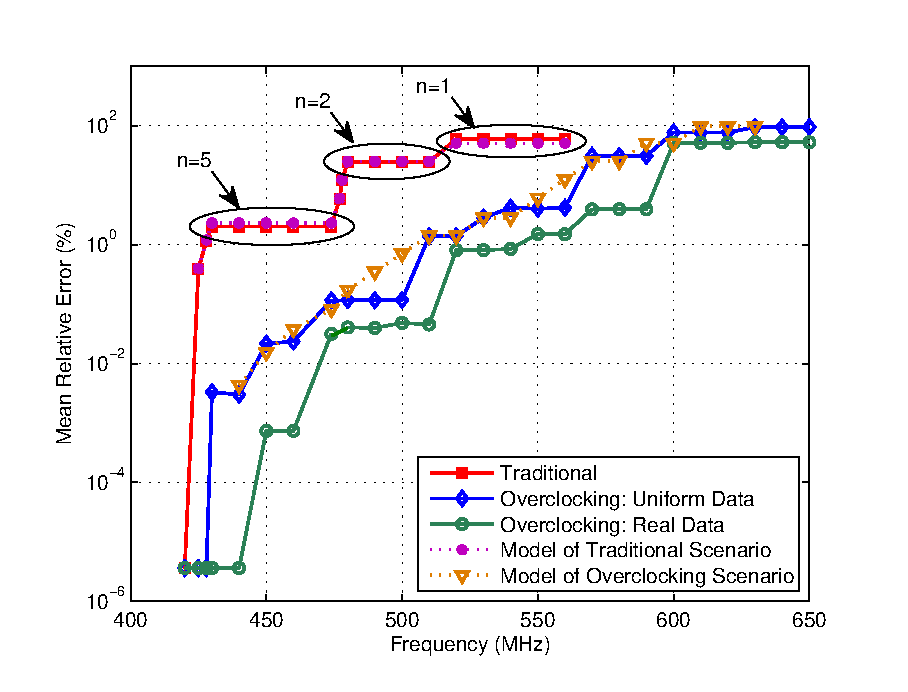
\includegraphics[width=3.5in]{./Figures/Exp/FIR/FIR_Compare_color.eps}
  \vspace{-2ex}
  \caption{A demonstration of two design perspectives with a $5^{th}$~order FIR filter, which is implemented on Virtex-6 FPGA. The modeled values of both overclocking errors and truncation errors are presented as dotted lines. The actual FPGA measurements are depicted using solid lines. Two types of inputs are employed in the overclocking scenario: the uniformly distributed data and the real image data from Lena.}
  \label{Fig:FIR}
\end{figure}

\begin{figure}[ht]
  \vspace{-2ex}
  % 425M, 450M, 480M, 520M
  \centering
  \subfigure[\scriptsize n=8,~SNR=47.97dB.]{
    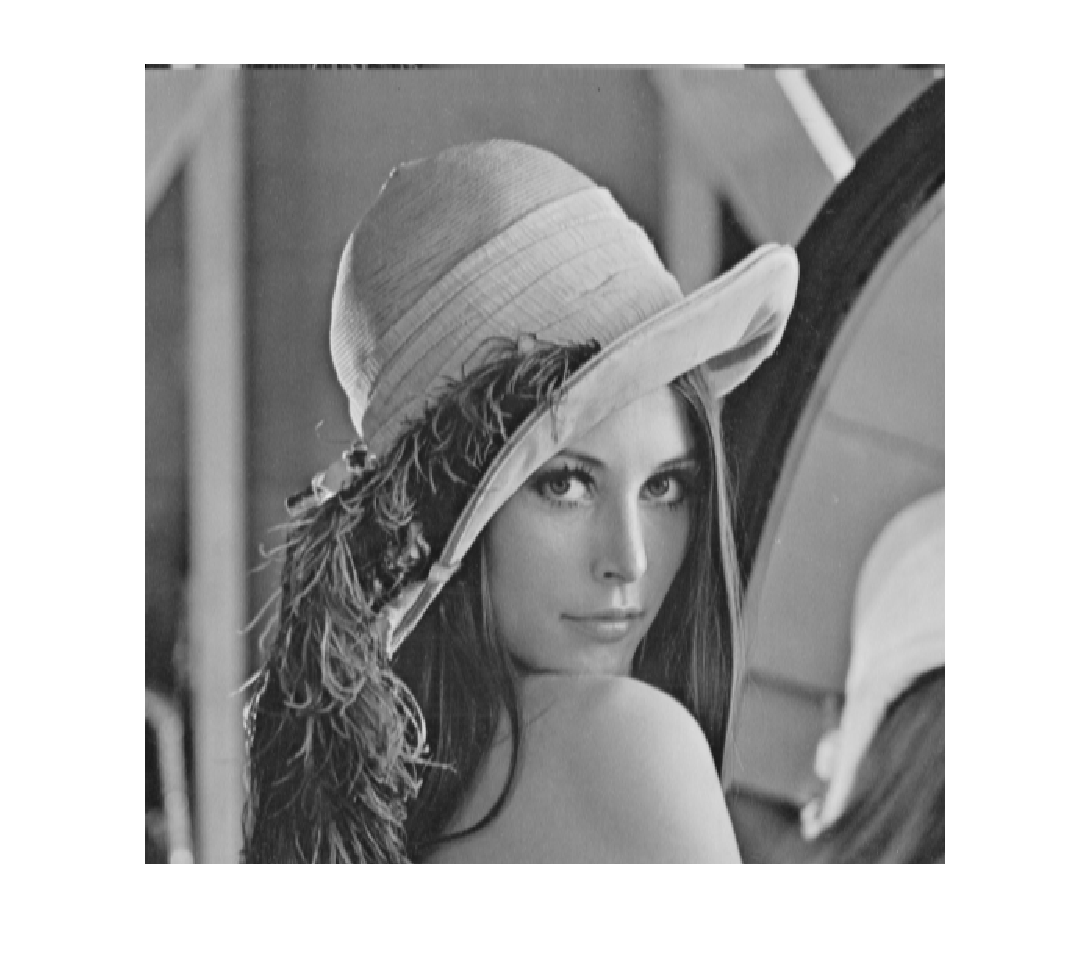
\includegraphics[width=.24\textwidth]{./Figures/Exp/FIR/LenaImages/FIRLena_T8.eps}
  }% This is important! use % to indicate same line, otherwise new line
  \subfigure[\scriptsize n=8,~SNR=44.94dB.]{
    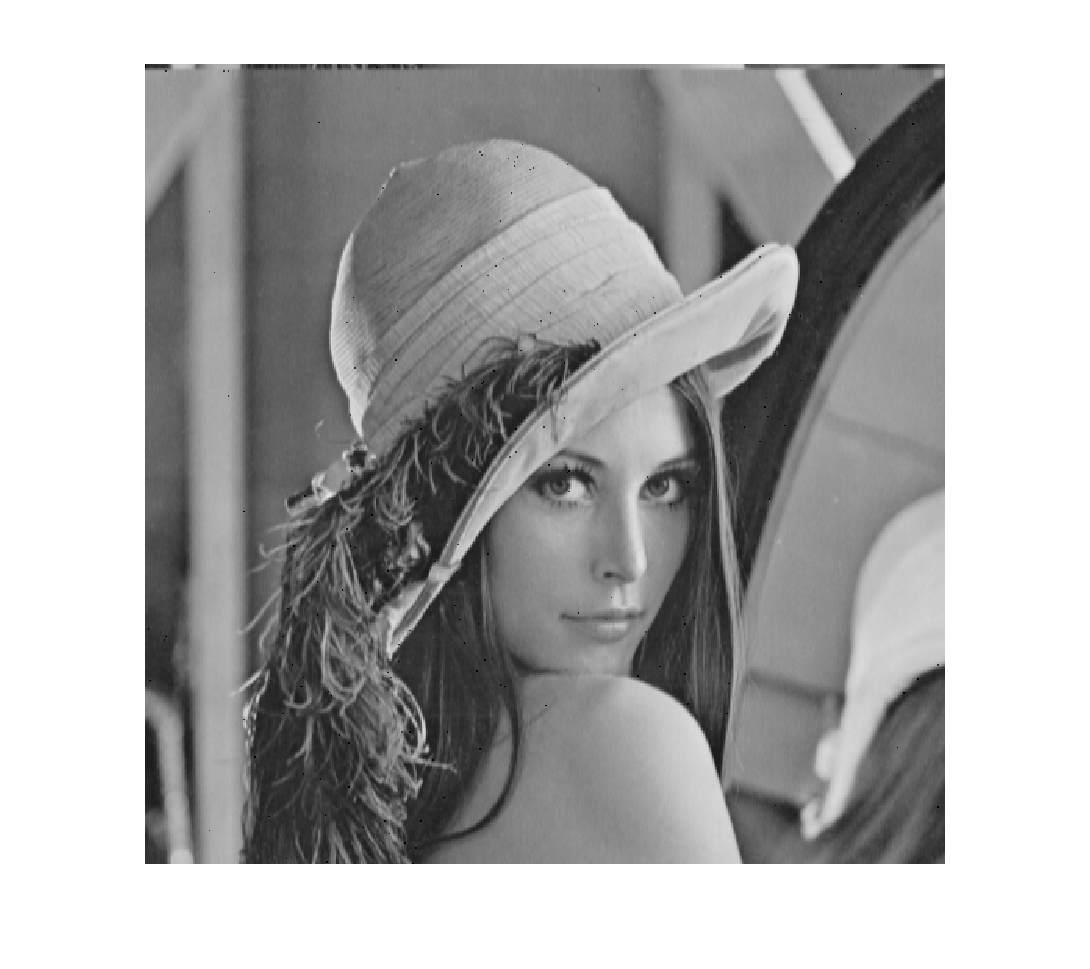
\includegraphics[width=.24\textwidth]{./Figures/Exp/FIR/LenaImages/FIRLena_T65.eps}
  }%
  \subfigure[\scriptsize n=8,~SNR=21.58dB.]{
    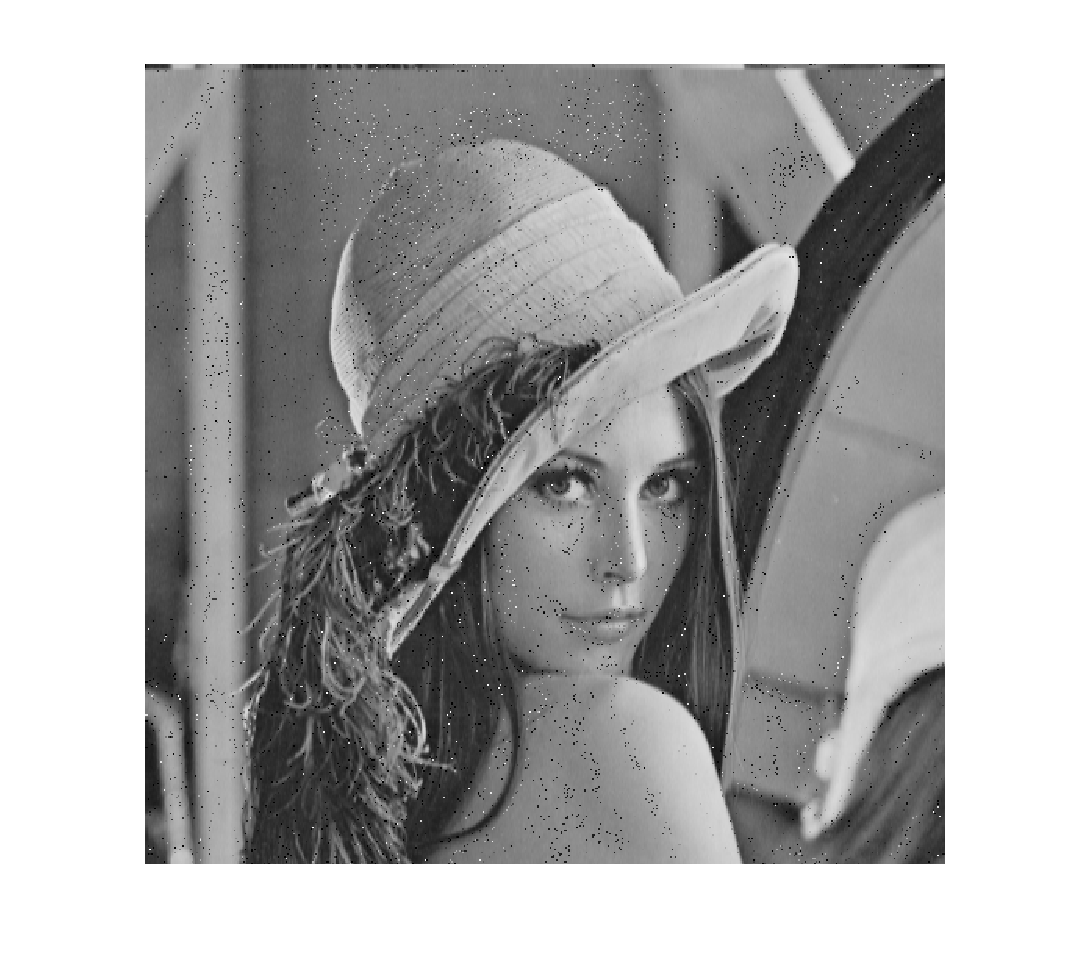
\includegraphics[width=.24\textwidth]{./Figures/Exp/FIR/LenaImages/FIRLena_T62.eps}
  }%
  \subfigure[\scriptsize n=8,~SNR=10.03dB.]{
    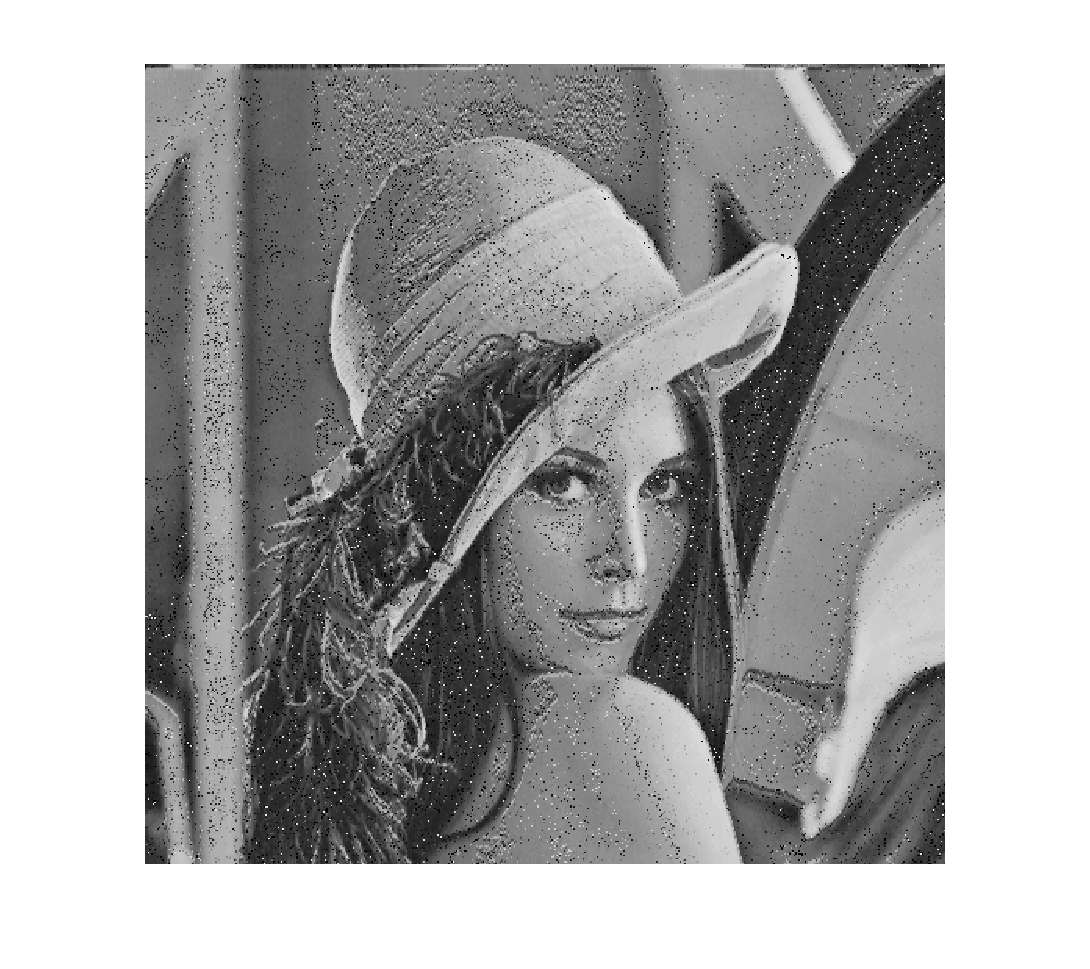
\includegraphics[width=.24\textwidth]{./Figures/Exp/FIR/LenaImages/FIRLena_T6.eps}
  }
  \subfigure[\scriptsize n=7,~SNR=26.02dB.]{
    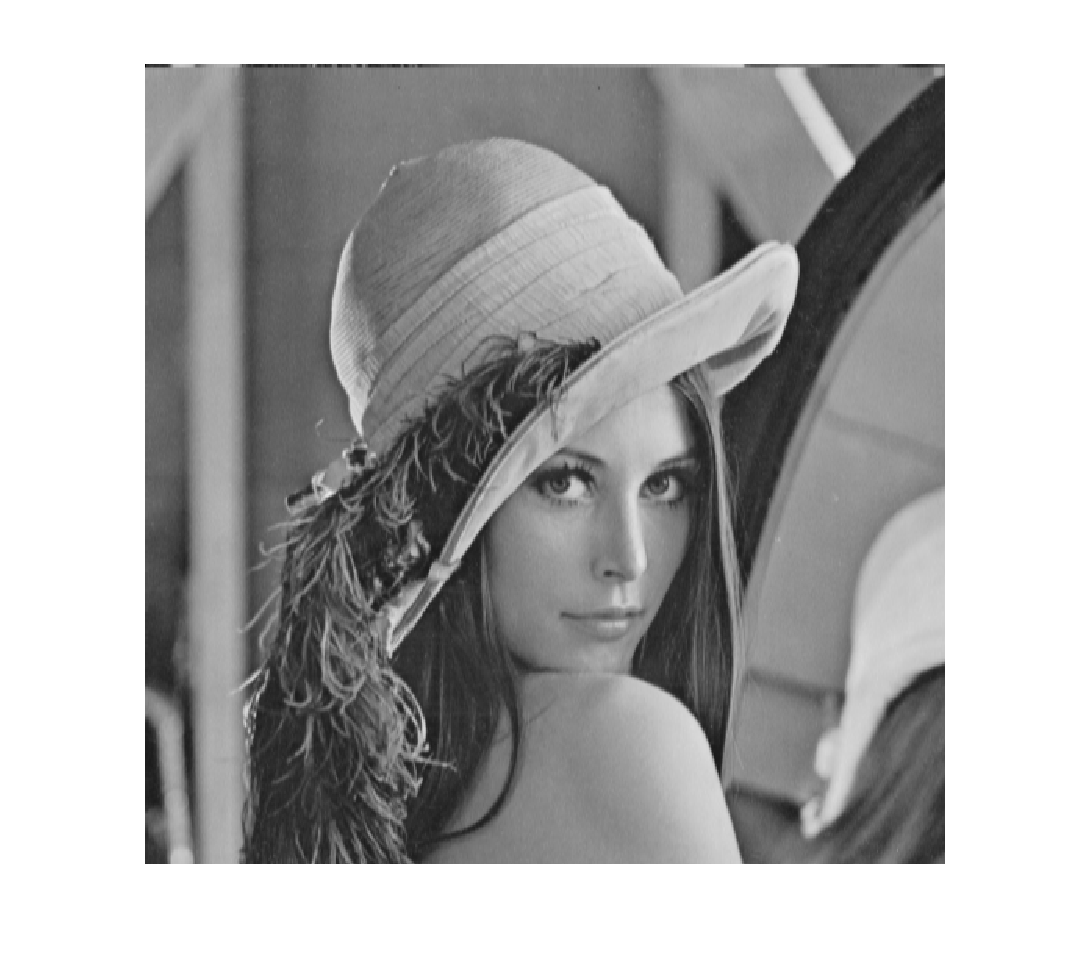
\includegraphics[width=.24\textwidth]{./Figures/Exp/FIR/LenaImages/FIRLena_Q7T10.eps}
  }% This is important! use % to indicate same line, otherwise new line
  \subfigure[\scriptsize n=5,~SNR=21.76dB.]{
    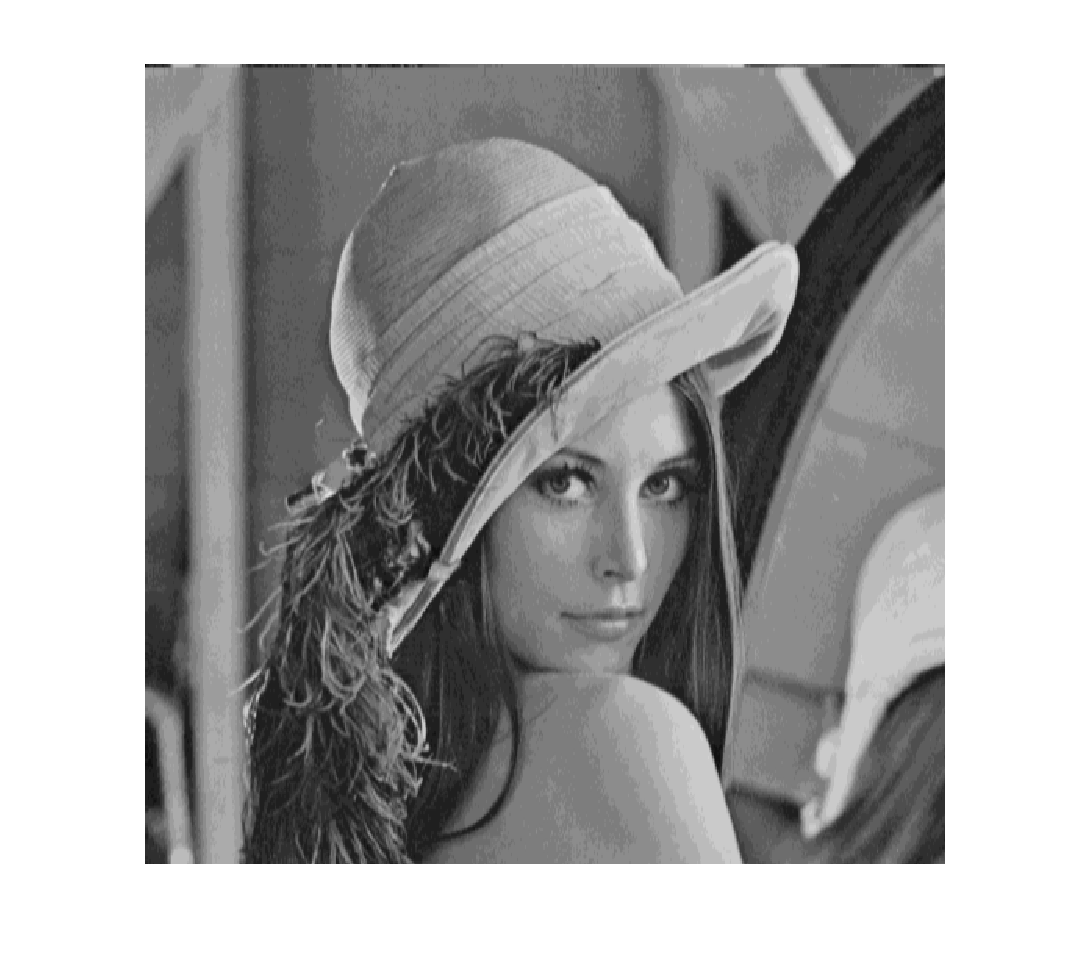
\includegraphics[width=.24\textwidth]{./Figures/Exp/FIR/LenaImages/FIRLena_Q4T10.eps}
  }%
  \subfigure[\scriptsize n=2,~SNR=6.57dB.]{
    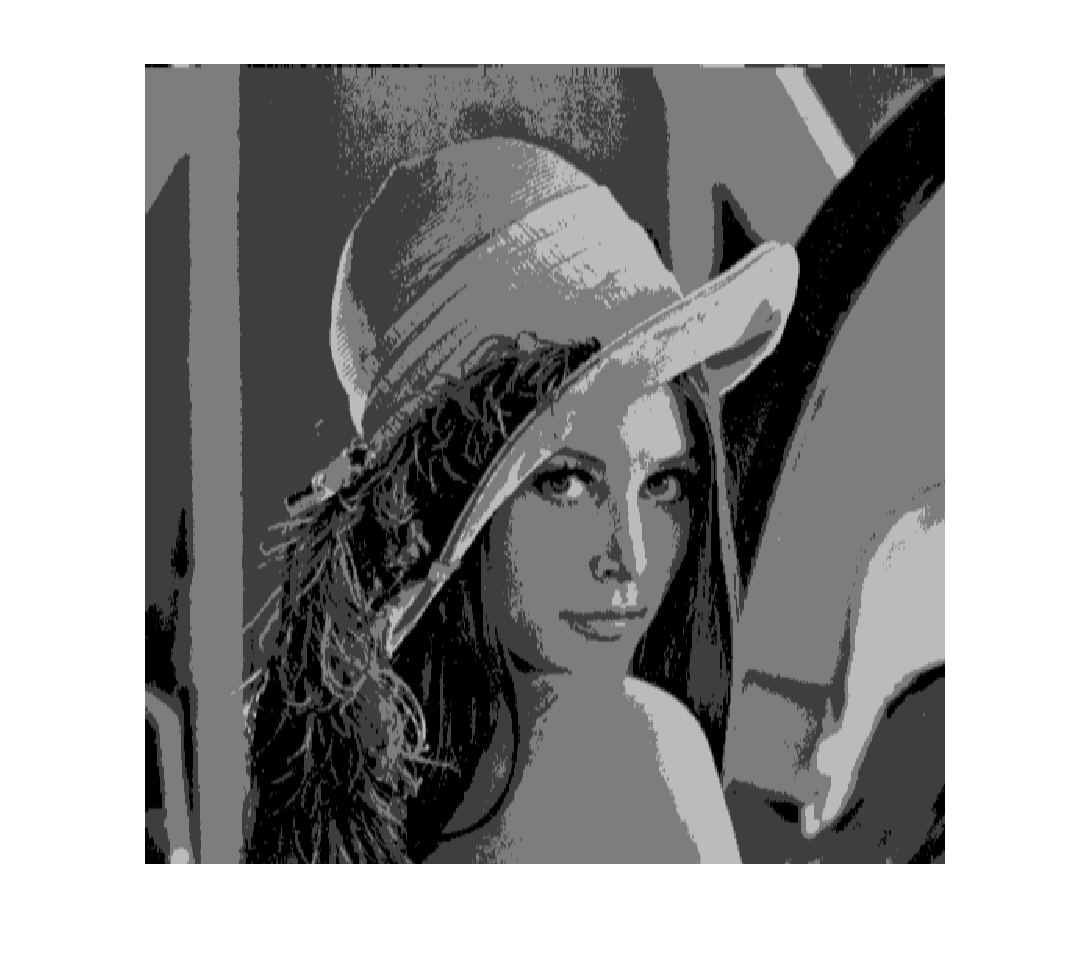
\includegraphics[width=.24\textwidth]{./Figures/Exp/FIR/LenaImages/FIRLena_Q2T10.eps}
  }%
  \subfigure[\scriptsize n=1,~SNR=3.95dB.]{
    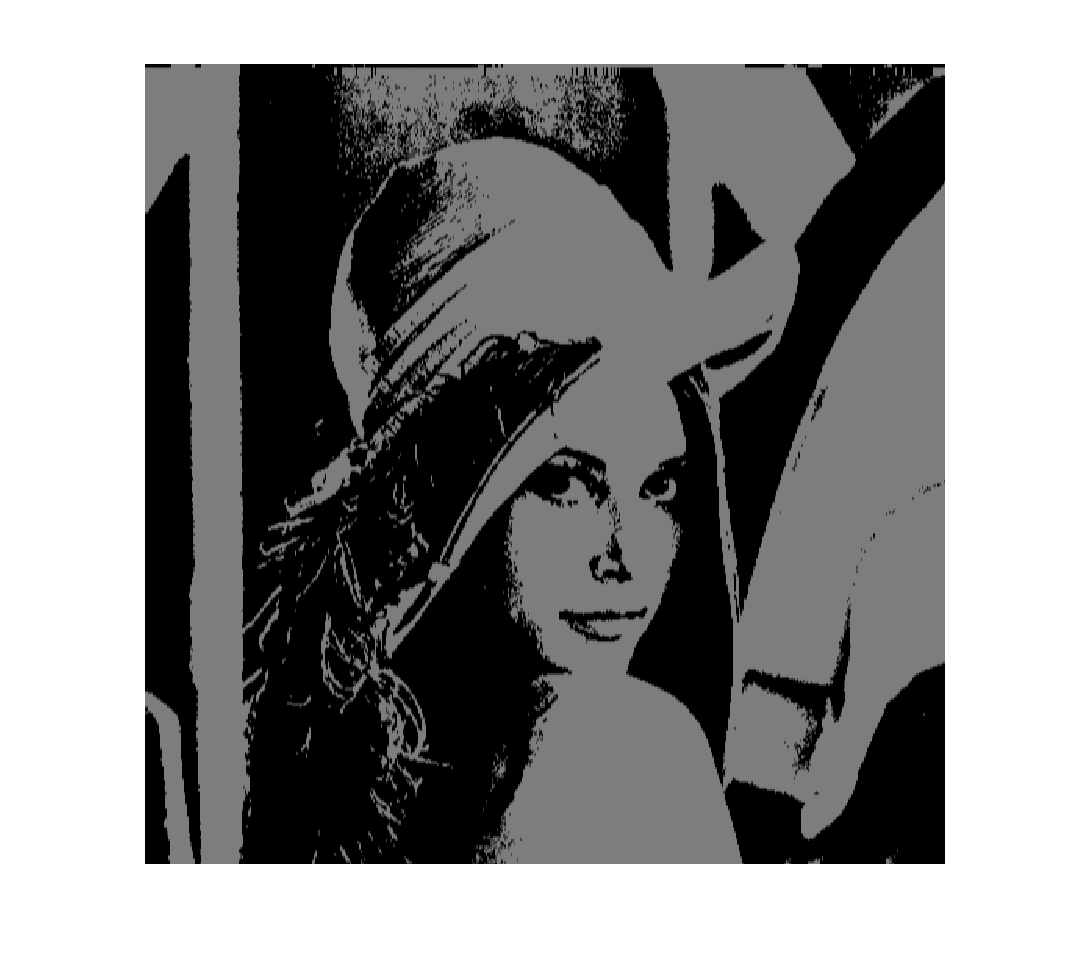
\includegraphics[width=.24\textwidth]{./Figures/Exp/FIR/LenaImages/FIRLena_Q1T10.eps}
  }
\vspace{-2ex}
\caption{Output images of the FIR filter for both overclocking scenario (top row) and traditional scenario (bottom row) when operating frequencies are $425MHz$, $450MHz$, $480MHz$ and $520MHz$ respectively (from left to right).}
\label{Fig:FIR_Lena}
\vspace{-1.5ex}
\end{figure}

According to Fig.~\ref{Fig:FIR}, output errors are reduced in the overclocking scenario for both input types in comparison to the traditional scenario, as the analytical model validates. In addition, we see that using real data, more significant reduction of $MRE$ are achieved, and that no errors are observed when frequency is initially increased. This is because for real data, long carry chains are typically generated with even smaller probabilities, and the longest carry chain rarely occurs.

The output images of the FIR filter for both of the two scenarios with increasing frequencies are presented in Fig.~\ref{Fig:FIR_Lena}, from which we can clearly see the differences between the errors generated in these two scenarios. In the overclocking scenario, we observe errors in the MSBs for certain input patterns. This leads to ``salt and pepper noise'', as shown on the images in the top row of Fig.~\ref{Fig:FIR_Lena}. In the traditional scenario, truncation causes an overall degradation of the whole image, as can be seen in the bottom row of Fig.~\ref{Fig:FIR_Lena}. Furthermore, it is worth noting that recovering from the latter type of error is more difficult, since it is generated due to precision loss.

%it is difficult to recover from the latter type of error, since it is generated due to precision loss.

In addition, we record the probability distribution of different length of carry chains using an 8-bit RCA with both data types, as shown in Fig.~\ref{Fig:CarryDistribution}. As the input data is 8-bit, the longest possible carry chain is of length 9-bit. It can be observed that when using Lena data,  the probability is only higher for carry chain with a length of 3-bit. While in other situations, using uniform data leads to higher probability, especially for long carry chain length. This finding explicitly demonstrates that longer carry chains happens with an even smaller probability when utilizing real data.
%
\begin{figure}[tbp]
  \centering
  \vspace{-2ex}
  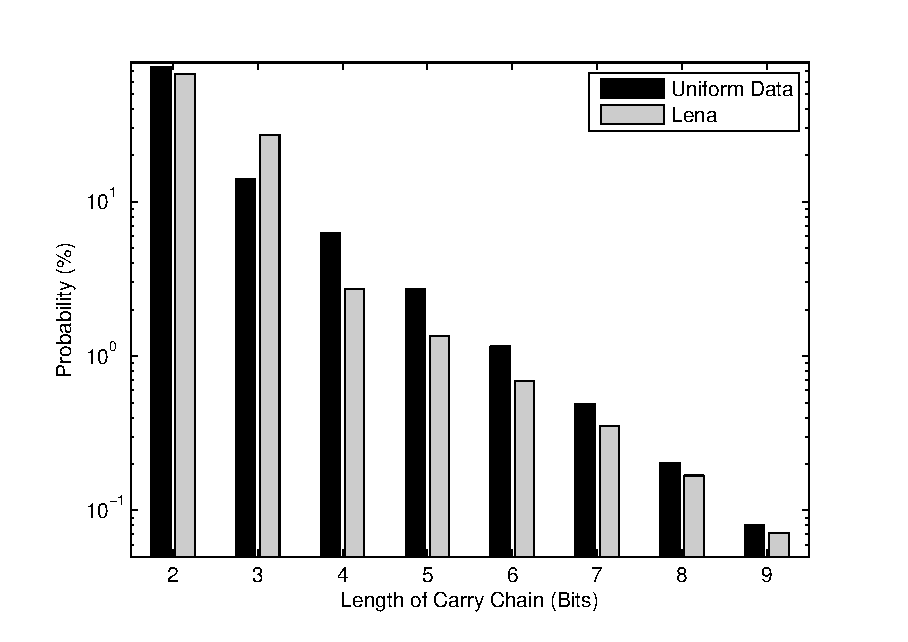
\includegraphics[width=3.5in]{./Figures/CC_length3.eps}
  \vspace{-1.5ex}
  \caption{Probability distribution of different length of carry chains in a 8-bit RCA. For the uniform data, two inputs of RCA are randomly sampled from a uniform distribution. For the image data Lena, one input of RCA uses the original data and the other uses the delayed original data for several clock cycles.}
  \label{Fig:CarryDistribution}
  \vspace{-1ex}
\end{figure}

\subsection{Potential Benefits in Datapath Design}
As we mentioned in Section~\ref{Section_OptimumAdder}, our results could be of interest to a circuit designer in two ways. Typically, either the designer will want to create a circuit that can run at a given frequency with the minimum possible $MRE$, or the algorithm designer will wish to run as fast as possible whilst maintaining a specific error tolerance. For the first design target, the experimental results for all five example designs on FPGA are summarized in Table~\ref{Table:Ratio_MRE} in terms of the relative reduction of $MRE$ as given in~(\ref{Eq:Relative_Reduction_MRE}) where $MRE_{Trad}$ and $MRE_{ovrc}$ denote the value obtained in the traditional scenario and in the overclocking scenario, respectively.
%
\begin{eqnarray}\label{Eq:Relative_Reduction_MRE}
  \frac{MRE_{Trad}-MRE_{ovrc}}{MRE_{Trad}}\times 100\%
\end{eqnarray}

In this table, the frequency is normalized to the maximum error-free frequency for each design when the input signal is 8-bit. The N/A in Table~\ref{Table:Ratio_MRE} refers to the situations where a certain frequency simply cannot be achieved using the traditional scenario. It can be seen that a significant reduction of $MRE$ can be achieved using the proposed overclocking scenario, and the geometric mean reduction varies from $67.9\%$ to $95.4\%$ using uniform input data. Even larger differences of $MRE$ can be observed when testing with real image data for each design, ranging from $83.6\%$ to $98.8\%$, as expected given the results shown in Fig.~\ref{Fig:FIR}.
%
\begin{table*}[tbp]
\vspace{-1ex}
 %% increase table row spacing, adjust to taste
   \renewcommand{\arraystretch}{1.05}
   \setlength{\tabcolsep}{3.5pt}
   \tbl{Relative Reduction of MRE ($\%$) in Overclocking Scenario for Various Normalized Frequencies Based on~(\ref{Eq:Relative_Reduction_MRE}) for Two Types of Input Data: Uniform Data (Uni) and Real Image Data from Lena (Lena).}{
   \centering
   %\footnotesize
   \scriptsize
   %\vspace{-4mm}
   \begin{threeparttable}
   \begin{tabular}{|c|cc|cc|cc|cc|cc||cc|}
     \hline
     \multirow{2}*{\begin{tabular}{c}\textbf{Normalized}\\\textbf{Frequency}\end{tabular}} &
     \multicolumn{2}{c|}{\textbf{FIR}} &
     \multicolumn{2}{c|}{\textbf{Sobel}} &
     \multicolumn{2}{c|}{\textbf{IIR}} &
     \multicolumn{2}{c|}{\textbf{Butterworth}} &
     \multicolumn{2}{c||}{\textbf{DCT4}} &
     \multicolumn{2}{c|}{\textbf{Geo.Mean}}\\
     &  {Uni} & {Lena } &  {Uni} & {Lena } &  {Uni} & {Lena }
     &  {Uni} & {Lena } &  {Uni} & {Lena } &  {Uni} & {Lena }\\
     \hline
     1.04 & 99.85	& 100.00  & 99.51 &	99.74 &	 72.28 &	90.09 &	 79.03 &	 100.00 &	 83.58 &	 98.06 & 86.14 & 97.50\\
     1.08 & 98.93	& 99.97   & 96.26 &	93.75 &	 71.64 &	90.50 &	 78.81 &	 100.00 &	 83.26 &	 98.45 & 85.15 & 96.46\\
     1.12 & 94.27	& 98.82   & 96.25 &	93.62 &	 73.63 &   88.25 &	 81.88 &	 84.87  &	 89.44 &	 99.56 & 86.68 & 92.84\\
     1.16 & 99.66	& 99.91   & 73.73 &	93.62 &	 73.10 &   89.92 &	 79.30 &	 84.23  &	 79.07 &	 99.44 & 80.44 & 93.23\\
     1.20 & 96.03	& 99.90   & 81.55 &	81.52 &	 70.76 &	75.67 &	 64.96 &	 84.50  &	 N/A\tnote{*}	  & N/A\tnote{*} & 77.46 & 84.95 \\
     1.24 & 98.46	& 99.32   & 81.43 &	81.67 &	 70.47 &	76.12 &	 63.66 &	 84.23  &	 N/A\tnote{*}	  & N/A\tnote{*} & 77.44 & 84.92\\
     1.28 & 95.39	& 99.29   & 60.41 &	78.24 &	 N/A\tnote{*}	    &   N/A\tnote{*}     &	54.38 &	 75.15  &	 N/A\tnote{*}	  & N/A\tnote{*} & 67.92 & 83.58\\
     1.32 & 95.37	& 98.75   & N/A\tnote{*}	  &	 N/A\tnote{*}	    &	 N/A\tnote{*}	    &	 N/A\tnote{*}   & N/A\tnote{*}   & N/A\tnote{*}    &    N/A\tnote{*}   & N/A\tnote{*} & 95.37	& 98.75 \\
     \hline
   \end{tabular}
   \normalsize
   \begin{tablenotes}
   \scriptsize
    \item[*] Current frequency cannot be achieved in the traditional scenario. These points are excluded from the calculation of geometric means.
   \end{tablenotes}
   \end{threeparttable}}
   \label{Table:Ratio_MRE}
 %\vspace{-1ex}
 \end{table*}

Table~\ref{Table:Max_Frequency} illustrates the frequency speedups for each design when the specified error tolerance varies from 0.05\% to 50\%. For all designs, we see that the overclocking scenario still outperforms the traditional scenario for each $MRE$ budget in terms of operating frequency. Likewise, the frequency speedup is higher for real image inputs than uniform inputs. The geometric mean of frequency speedups of $3.07\%$ to $21.8\%$ can be achieved by using uniform data, with $5.32\%$ to $27.6\%$ when using real image data.
%
\begin{table*}[tbp]
\vspace{-1ex}
 %% increase table row spacing, adjust to taste
   \renewcommand{\arraystretch}{1.05}
   \setlength{\tabcolsep}{3.5pt}
   \tbl{Frequency Speedups ($\%$) in Overclocking Scenario Under Various Error Budgets for Two Types of Input Data: Uniform Data (Uni) and Real Image Data from Lena (Lena).}{
%   \vspace{-2ex}
   \label{Exp_Real_Inputs}
   \centering
   %\footnotesize
   \scriptsize
   \begin{tabular}{|c|cc|cc|cc|cc|cc||cc|}
     \hline
     \multirow{2}*{\begin{tabular}{c}\textbf{Error}\\\textbf{Budget($\%$)}\end{tabular}} &
     \multicolumn{2}{c|}{\textbf{FIR}} &
     \multicolumn{2}{c|}{\textbf{Sobel}} &
     \multicolumn{2}{c|}{\textbf{IIR}} &
     \multicolumn{2}{c|}{\textbf{Butterworth}} &
     \multicolumn{2}{c||}{\textbf{DCT4}} &
     \multicolumn{2}{c|}{\textbf{Geo.Mean}} \\
     %\multirow{2}*{\begin{tabular}{c}\textbf{Geo.}\\\textbf{Mean}\end{tabular}}\\
     & {Uni} & {Lena } &  {Uni} & {Lena } &  {Uni} & {Lena }
     & {Uni} & {Lena } &  {Uni} & {Lena } &  {Uni} & {Lena }\\
     \hline
     0.05 & 4.76 &	21.43&	 6.82&	6.82&	0.95&	 1.26&	12.40&	 24.03&	 0.72&	 0.96  &3.07 & 5.32\\
     0.5  & 19.05&	21.43&	 13.64&	6.82&	0.63&	 10.06&	24.03&	 24.03&	0.48&	 12.44   &4.52 &13.45\\
     1    & 19.05&	28.57&	 13.64&	18.18&	 10.06&	16.35&	 24.03&	 24.03&	 0.48&	 12.44    &7.86 &19.10\\
     5    & 19.15&	25.53&	 18.18&	18.18&	 0.54&	0.82&	 0.63&	 0.94&	 7.66&	 12.44    &3.91    &5.36\\
     10   & 19.15&	25.53&	 10.64&	10.64&	 0.54&	1.09&	 6.92&	 13.21&	 4.91&	 4.911  &5.19  &7.19\\
     20   & 19.15&	25.53&	 5.77&	15.39&	 8.70&	8.70&	 3.26&	 3.26&	 6.70&	 10.88    &7.32    &10.39\\
     50   & 15.69&	15.69&	 10.53&	19.30&	 42.50&	50.00&	 46.74&	 54.89&	 15.06&	 19.25    &21.8 &27.59\\
     \hline
   \end{tabular}}
   \normalsize
   \label{Table:Max_Frequency}
   \vspace{-1ex}
 \end{table*}


\subsection{Area Overhead of Our Approach}
For both aforementioned design goals, it should be noted that an extra benefit of using the traditional approach is that reducing datapath precision would potentially lead to a smaller design, in comparison to our proposed overclocking scenario. Consequently, the area overheads of our approach are summarized in Table~\ref{Table:AreaFrequency} and Table~\ref{Table:AreaError} for both design goals. In our experiments, the area overhead is evaluated in terms of the number of LUTs and Slices in the FPGA technology, while similar metrics can also be employed if applying our approach into other hardware platforms. It can be seen that for a given frequency requirement with minimum possible errors (Table~\ref{Table:AreaFrequency}), the geometric mean of area overhead ranges from $1.16\times$ and $1.15\times$ to $5.57\times$ and $4.46\times$ for LUTs and Slices, respectively. This result illustrates that although using traditional approach would lead to smaller design, the area benefits are less attractive than the performance or accuracy benefits brought by utilizing the proposed new approach, especially for relaxed frequency requirements.

An even smaller area overhead can be found for a specified error budget with the maximum clock frequencies. As seen in Table~\ref{Table:AreaError}, the geometric mean of area overhead in terms of LUTs and Slices is $1.00\times\sim4.67\times$ and $1.00\times\sim3.70\times$ respectively. Notice that an area overhead of $1\times$ means both the overclocking scenario and the traditional scenario use the original precision, however the former achieves frequency speedups as seen in Table~\ref{Table:AreaError}, because a specific error budget can be tolerated.

In general, a very small area overhead of our approach can be observed when the design is initially operated beyond the safe region with higher frequencies or with a small error budget (e.g. $\sim10\%$). In addition at even higher operating frequencies or larger error specifications, our approach achieves large performance or accuracy improvements at a cost of a relatively small extra area.
%
\begin{table*}[tbp]
\vspace{-2ex}
 %% increase table row spacing, adjust to taste
   \renewcommand{\arraystretch}{1.05}
   \setlength{\tabcolsep}{3.5pt}
   \tbl{Area Overhead of Our Approach with respect to Given Frequency Requirements}{
   \centering
   %\footnotesize
   \scriptsize
   \begin{threeparttable}
   \begin{tabular}{|c|cc|cc|cc|cc|cc||cc|}
     \hline
     \multirow{2}*{\begin{tabular}{c}\textbf{Normalized}\\\textbf{Frequency}\end{tabular}} &
     \multicolumn{2}{c|}{\textbf{FIR}} &
     \multicolumn{2}{c|}{\textbf{Sobel}} &
     \multicolumn{2}{c|}{\textbf{IIR}} &
     \multicolumn{2}{c|}{\textbf{Butterworth}} &
     \multicolumn{2}{c||}{\textbf{DCT4}} &
     \multicolumn{2}{c|}{\textbf{Geo.Mean}}\\
     &  {\scriptsize LUTs} & {\scriptsize Slices } &  {\scriptsize LUTs} & {\scriptsize Slices } &  {\scriptsize LUTs} & {\scriptsize Slices }
     &  {\scriptsize LUTs} & {\scriptsize Slices } &  {\scriptsize LUTs} & {\scriptsize Slices } &  {\scriptsize LUTs} & {\scriptsize Slices}\\
     \hline
     1.04 & 1.24	& 1.05  & 1.12 &	1.22 &	 1.26 &	1.42 &	 1.16 &	 1.11 &	 1.13 &	 1.00 & 1.18 & 1.15\\
     1.08 & 1.24	& 1.05	& 1.03 &	1.08 &	 1.26 &	1.42 &	 1.16 &	 1.11 &	 1.11 &	 1.15 & 1.16 & 1.16\\
     1.12 & 1.24	& 1.05   & 1.03 &	1.08 &	 1.26 & 1.42 &	 1.37 &	1.54  &	 2.30 &	 2.17 & 1.38 & 1.40\\
     1.16 & 2.95	& 2.56   & 1.03 &	1.08 &	 1.61 & 1.71 &	 1.99 &	 2.03  &	 4.60 &	 2.89 &2.14 & 1.95\\
     1.20 & 2.95	& 2.56   & 1.66 &	1.39 &	 2.77 &	3.48 &	3.17 &	 3.50  &	 N/A\tnote{*}	  & N/A\tnote{*} & 2.56 & 2.57 \\
     1.24 & 4.42	& 3.15  & 4.00 &	3.55 &	 7.87 &	6.73 &	6.92 &	 5.25  &	 N/A\tnote{*}	  & N/A\tnote{*} & 5.57 & 4.46\\
     1.28 & 4.42	& 3.15   & 4.00 &	3.55 &	 N/A\tnote{*}	    &   N/A\tnote{*}     &	6.92 &	 5.25  &	 N/A\tnote{*}	  & N/A\tnote{*} & 4.97& 3.89\\
     1.32 & 4.42	& 3.15   & N/A\tnote{*}	  &	 N/A\tnote{*}	    &	 N/A\tnote{*}	    &	 N/A\tnote{*}   & N/A\tnote{*}   & N/A\tnote{*}    &    N/A\tnote{*}   & N/A\tnote{*} & 4.42	& 3.15 \\
     \hline
   \end{tabular}
   \normalsize
   \begin{tablenotes}
   \scriptsize
    \item[*] Current frequency cannot be achieved in the traditional scenario. These points are excluded from the calculation of geometric means.
   \end{tablenotes}
   \end{threeparttable}}
   \label{Table:AreaFrequency}
 \end{table*}
%
 \begin{table*}[tbp]
 \vspace{-1ex}
 %% increase table row spacing, adjust to taste
   \renewcommand{\arraystretch}{1.05}
   \setlength{\tabcolsep}{3.5pt}
   \tbl{Area Overhead of Our Approach with respect to Given Error Budgets.}{
   \centering
   %\footnotesize
   \scriptsize
   \begin{tabular}{|c|cc|cc|cc|cc|cc||cc|}
     \hline
     \multirow{2}*{\begin{tabular}{c}\textbf{Error}\\\textbf{Budget($\%$)}\end{tabular}} &
     \multicolumn{2}{c|}{\textbf{FIR}} &
     \multicolumn{2}{c|}{\textbf{Sobel}} &
     \multicolumn{2}{c|}{\textbf{IIR}} &
     \multicolumn{2}{c|}{\textbf{Butterworth}} &
     \multicolumn{2}{c||}{\textbf{DCT4}} &
     \multicolumn{2}{c|}{\textbf{Geo.Mean}} \\
     %\multirow{2}*{\begin{tabular}{c}\textbf{Geo.}\\\textbf{Mean}\end{tabular}}\\
     & {\scriptsize LUTs} & {\scriptsize Slices } &  {\scriptsize LUTs} & {\scriptsize Slices } &  {\scriptsize LUTs} & {\scriptsize Slices }
     & {\scriptsize LUTs} & {\scriptsize Slices } &  {\scriptsize LUTs} & {\scriptsize Slices } &  {\scriptsize LUTs} & {\scriptsize Slices }\\
     \hline
     0.05 & 1.00&	1.00& 1.00&	1.00& 1.00&	 1.00&	1.00&	 1.00&	1.00&	 1.00  &1.00  &  1.00\\
     0.5  & 1.02&	1.15& 1.00&	1.00& 1.00&	 1.00&	1.00&	 1.00&	1.00&	 1.00   &1.00 &1.03\\
     1    & 1.02&	1.15& 1.00&	1.00& 1.00&	 1.00&	1.00&	 1.00&	1.00&	 1.00   &1.00 &1.03\\
     5    & 1.24&	1.05& 1.00&	1.00& 1.26&   1.42&   1.65&   1.11&	 1.00&    1.00   &1.13    &1.11\\
     10   & 1.24&	1.05& 1.12&	1.22& 1.26&	1.42& 1.65&	1.11& 1.11&	 1.15&    1.18    &1.18\\
     20   & 1.24&	1.05& 1.03&	1.08& 1.26&	1.42& 6.92&	 5.25&   3.45&	 2.17   &2.07    &1.79\\
     50   & 2.95&	2.56& 4.00&	3.55& 7.87&	6.73& 6.92&	 5.25&   3.45&	 2.12	&4.67 &3.70\\
     \hline
   \end{tabular}}
   \normalsize
   \label{Table:AreaError}
 \end{table*}



\section{Conclusion}  \label{Section_Conclusion}
In this paper, we have explored the probabilistic behavior of key arithmetic primitives in an FPGA when operating beyond the deterministic region. Two design scenarios that might generate errors: violating timing constraints and reducing precisions, have been investigated. It has been found that simply allowing timing violations to happen would potentially lead to either reductions in average errors or speedups in clock frequencies, in comparison to the traditional approach where the target timing is met by limiting the precisions throughout the datapath. To verify this hypothesis, probabilistic models have been developed for errors generated from both design methodologies, and empirical results on a Virtex-6 FPGA have also been obtained over a set of DSP applications. Besides, the silicon area has also been taken into account for the trade-offs. We have shown that applying our approach on basic arithmetic primitives would potentially outperform utilizing the traditional approach on either the same architectures or structures specifically designed for high performance, of which the precision loss is even greater under a tight area budget.

While this research has shown a promising direction for sustaining performance scaling, in the future we wish to extend the current model by considering the propagation of error through arithmetic circuits at the component level, and to apply this approach beyond datapath designs with a variety of PVT variations.

%apply this approach onto arithmetic units based on alternative number representations, and explore the probabilistic behavior of these operators under a variety of process, voltage and temperature variations.



%While this research has shown a promising direction for sustaining performance scaling, there are several issues that would be of interest for future research. A critical finding from this work is the direction inconsistency between carry propagation (from the LSB to the MSB) and results sampling (from the MSB to the LSB). In this case, although the probability of generating overclocking errors might be small, the magnitude of error is large, which restricts the performance improvement to a large extent. Another limitation is that the inputs of current designs are applied digits by digits, while the correct outputs are updated based on a bit-serial fashion due to the delay of carry propagation.  To tackle this problem, we wish to investigate non-conventional arithmetic operations and data representations. One possible candidate is known as ``online arithmetic ''~\cite{Ercegovac_Overview,Ercegovac_Book}, in which the computation is performed bit-serially from the MSB to the LSB. This potentially fill the gap of the aforementioned direction inconsistencies. In addition, an alternative number representation metric by using redundant numbers could be employed to largely reduce the lengths of carry chains. While research in this area mainly focus on the ASIC domain~\cite{RedundantMult_1985,RedundantMult_1987}, it is worthwhile exploring the potential benefits and overheads when employing this method using our approach.

%, and this data representation metric has been utilized in ASIC designs

%and carry propagation can be nearly removed because a redundant number system [xxx] is used to represent numbers. Therefore it is worthwhile exploring the potential benefits and overheads when employing this method in our approach.





% Figure
%\begin{figure}
%\centerline{\includegraphics{acmsmall-mouse}}
%\caption{Code before preprocessing.}
%\label{fig:one}
%\end{figure}

%\begin{figure}
%  \centering
%  \includegraphics[width=\textwidth]{./acmsmall-mouse.eps}
%  \caption{Figure}

% Table
%\begin{table}%
%\tbl{Simulation Configuration\label{tab:one}}{%
%\begin{tabular}{|l|l|}
%\hline
%TERRAIN{$^a$}   & (200m$\times$200m) Square\\\hline
%Node Number     & 289\\\hline
%Node Placement  & Uniform\\\hline
%Application     & Many-to-Many/Gossip CBR Streams\\\hline
%Payload Size    & 32 bytes\\\hline
%Routing Layer   & GF\\\hline
%MAC Layer       & CSMA/MMSN\\\hline
%Radio Layer     & RADIO-ACCNOISE\\\hline
%Radio Bandwidth & 250Kbps\\\hline
%Radio Range     & 20m--45m\\\hline
%\end{tabular}}
%\begin{tabnote}%
%\Note{Source:}{This is a table
%sourcenote. This is a table sourcenote. This is a table
%sourcenote.}
%\vskip2pt
%\Note{Note:}{This is a table footnote.}
%\tabnoteentry{$^a$}{This is a table footnote. This is a
%table footnote. This is a table footnote.}
%\end{tabnote}%
%\end{table}%

% Acknowledgments
%\begin{acks}
%The authors would like to thank xxx.
%\end{acks}

% Bibliography
\bibliographystyle{ACM-Reference-Format-Journals}
%\bibliography{acmsmall-sample-bibfile}
\bibliography{Reference}
                             % Sample .bib file with references that match those in
                             % the 'Specifications Document (V1.5)' as well containing
                             % 'legacy' bibs and bibs with 'alternate codings'.
                             % Gerry Murray - March 2012

% History dates
%\received{February 2007}{March 2009}{June 2009}

% Electronic Appendix
\elecappendix

\medskip


\end{document}
% End of v2-acmsmall-sample.tex (March 2012) - Gerry Murray, ACM


